\documentclass[onecolumn, draftclsnofoot,10pt, compsoc]{IEEEtran}
\usepackage{graphicx}
\usepackage{url}
\usepackage{setspace}
\usepackage{indentfirst}
\usepackage{longtable}
\usepackage{pdfpages}

\usepackage{geometry}
\geometry{textheight=9.5in, textwidth=7in}

% 1. Fill in these details
\def \CapstoneTeamName{		    The Apolloers}
\def \CapstoneTeamNumber{		49}
\def \GroupMemberOne{			Jonathan Ropp}
\def \GroupMemberTwo{			Shannon Sandy}
\def \GroupMemberThree{			Dean Akin}
\def \CapstoneProjectName{		Apollo 11 3D Animation}
\def \CapstoneSponsorCompany{	OMSI}
\def \CapstoneSponsorPersona{	Jim Todd}
\def \CapstoneSponsorPersonb{	Mike Bailey}

% 2. Uncomment the appropriate line below so that the document type works
\def \DocType{		
                %Problem Statement
				%Requirements Document Draft
				%Technology Review
				%Design Document
				%Progress Report
				Project Hand Off
				}
			
\newcommand{\NameSigPair}[1]{\par
\makebox[2.75in][r]{#1} \hfil 	\makebox[3.25in]{\makebox[2.25in]{\hrulefill} \hfill		\makebox[.75in]{\hrulefill}}
\par\vspace{-12pt} \textit{\tiny\noindent
\makebox[2.75in]{} \hfil		\makebox[3.25in]{\makebox[2.25in][r]{Signature} \hfill	\makebox[.75in][r]{Date}}}}
% 3. If the document is not to be signed, uncomment the RENEWcommand below
\renewcommand{\NameSigPair}[1]{#1}

%%%%%%%%%%%%%%%%%%%%%%%%%%%%%%%%%%%%%%%
\begin{document}
\begin{titlepage}
    \pagenumbering{gobble}
    \begin{singlespace}
        \hfill 
        % 4. If you have a logo, use this includegraphics command to put it on the coversheet.
        \includegraphics[height=2cm]{OSU_horizontal_2C_O_over_B.eps}   
        \par\vspace{.2in}
        \centering
        \scshape{
            \huge CS Capstone \DocType \par
            {\large\today}\par
            \vspace{.5in}
            \textbf{\Huge\CapstoneProjectName}\par
            \vfill
            {\large Prepared for}\par
            \Huge \CapstoneSponsorCompany\par
            \vspace{5pt}
            {\Large\NameSigPair{\CapstoneSponsorPersona}\par}
            {\Large\NameSigPair{\CapstoneSponsorPersonb}\par}
            {\large Prepared by }\par
            Group\CapstoneTeamNumber\par
            % 5. comment out the line below this one if you do not wish to name your team
            \CapstoneTeamName\par 
            \vspace{5pt}
            {\Large
                \NameSigPair{\GroupMemberOne}\par
                \NameSigPair{\GroupMemberTwo}\par
                \NameSigPair{\GroupMemberThree}\par
            }
            \vspace{20pt}
        }
        \begin{abstract}
        % 6. Fill in your abstract   
    
During the 2018-19 school year, our Capstone group created a 3D animation of the Apollo 11 Moon Landing mission for use in the OMSI planetarium. This document is a compilation of all technical documentation that was created during the process, as well as conclusions from the team members. In short, we met many of our goals for this project and created an interactive animation in OpenGL, but more work is being done to translate our project into a format that can be used at OMSI. 

        \end{abstract}     
    \end{singlespace}
\end{titlepage}
\newpage
\pagenumbering{arabic}
\tableofcontents

%%%%%%%%%%%%%%%%%%%%%%%%%%%%%%%%%%%%%%%%%%%%%%%%%%%%%%%%%%%%%%%%%%%%%%%%%
%%%%%%%%%%%%%%%%%%%%%%%%%%%%%%%%%%%%%%%%%%%%%%%%%%%%%%%%%%%%%%%%%%%%%%%%%
\section{Introduction to Project}

During the 2018-2019 school year, our team worked on creating a 3-D animation of the  Apollo 11 Moon Landing. Jim Todd, the Director of Space Science Education at the Oregon Museum of Science and Industry (OMSI) requested this project for Summer 2019, which will mark the 50th anniversary of the moon landing. Our goal was to accurately depict the Apollo 11 mission in a way that was historically accurate, as well as creating something that would be engaging for all audiences at OMSI, ranging from young children to astrology experts. 

Three Senior Computer Science Majors formed our team: Dean Akin, Jonathan Ropp, and Shannon Sandy. Dean did keyframe animation as well as lighting on the Earth and Moon. Shannon did work on the audio clips, as well as the landing animations. She created the feathered landing site zoom animation as well as work and improve on lighting shaders. Jonathan created the flight path in its entirety, formulated the Bezier curves of the static path as well as the dynamic moving flight path through the use of the aforementioned keyframing animation class. Mike Bailey, a computer graphics professor at Oregon State University, mentored our group, which was coined \textit{The Apolloers}. Dr. Bailey's involvement was day to day, and he was present during a majority of the development of the animation and documentation, and has even contributed a significant amount to the development of the project in the form of pertinent information, technical support, and code contribution. Jim Todd also provided contextual information important to make the animation as authentic as possible while on the lunar surface. While we were only able to meet in person twice during this project, Jim always gave great feedback and gave us pointers to keep moving forward with the project. 

%Who requested it?
%Jim Todd, Director of Space Science Education at OMSI requested we make an animation about the Apollo 11 mission.
%Why was it requested?
%It was meant to be a commemoration of the feats that were achieved during the Apollo 11 mission. 
%What is its importance?
%It also will serve as a educational tool to teach about what we could achieve back then, and what we can achieve right now.
%Who was/were your client(s)?
%Jim Todd, Director of Space Education at OMSI, and Mike Bailey, Professor of Computer Science at Oregon State University.
%Who are the members of your team?
%Shannon Sandy, Jonathan Ropp, Dean A. Akin
%What were their roles?
%Dean did keyframe animation as well as lighting on the Earth and Moon. Shannon did work on the audio clips, as well as the landing animations. She created the feathered landing site zoom animation as well as work and improve on lighting shaders. Jonathan created the flight path in its entirety, formulated the bezier curves of the static path as well as the dynamic moving flight path through the use of the aformentioned keyframing animation class. 
%What was the role of the client(s)? (I.e., did they supervise only, or did they participate in doing development)
%We met with Jim Todd 2 times before, both times we were briefed on how the planetarium system worked as well as given examples of scripts written in their in-house scripting language, Dark-Matter. We use these scripts as references when we are transferring our project into a Dark-Matter native animation. Communication is limited due to distance and schedules, and because of this, Jim was not present during a majority of the development of the animation, but was present for all of the documentation and provided contextual information important to make the animation as authentic as possible. Dr. Bailey's involvement was day to day, and he was present during a majority of the development of the animation and documentation, and has even contributed a significant amount to the development of the project in the form of pertinent information, technical support, and code contribution. 
%%%%%%%%%%%%%%%%%%%%%%%%%%%%%%%%%%%%%%%%%%%%%%%%%%%%%%%%%%%%%%%%%%%%%%%%%
%%%%%%%%%%%%%%%%%%%%%%%%%%%%%%%%%%%%%%%%%%%%%%%%%%%%%%%%%%%%%%%%%%%%%%%%%
\section{Requirements doc}
\begin{titlepage}
    \pagenumbering{gobble}
    \begin{singlespace}
        \hfill 
        % 4. If you have a logo, use this includegraphics command to put it on the coversheet.
        \includegraphics[height=2cm]{OSU_horizontal_2C_O_over_B.eps}   
        \par\vspace{.2in}
        \centering
        \scshape{
            \huge CS Capstone Requirements Document \par
            {\large\today}\par
            \vspace{.5in}
            \textbf{\Huge\CapstoneProjectName}\par
            \vfill
            {\large Prepared for}\par
            \Huge \CapstoneSponsorCompany\par
            \vspace{5pt}
            {\Large\NameSigPair{\CapstoneSponsorPersona}\par}
            {\large Prepared by }\par
            Group\CapstoneTeamNumber\par
            % 5. comment out the line below this one if you do not wish to name your team
            \CapstoneTeamName\par 
            \vspace{5pt}
            {\Large
                \NameSigPair{\GroupMemberOne}\par
                \NameSigPair{\GroupMemberTwo}\par
                \NameSigPair{\GroupMemberThree}\par
            }
            \vspace{20pt}
        }
        \begin{abstract}
        % 6. Fill in your abstract    
        	Our group, The Apolloers, is working with Mike Bailey to create a 3D animation about the Apollo 11 Moon Landing. This animation will be put on display in OMSI during the Summer of 2019 for the 50th anniversary of the Apollo 11 mission. The project will allow viewers to see what it is like on the Moon through animated views placed throughout the scene. This document breaks the project into requirements that we will use to guide our project through the development process. 
        \end{abstract}     
    \end{singlespace}
\end{titlepage}
\newpage
\pagenumbering{arabic}
%\tableofcontents
\subsection*{Revisions}
\begin{tabular} {|p{3.25cm}|p{5cm}|p{7cm}|}
\hline
Section & Original & New \\ \hline
1.2 - Scope & \begin{itemize}
  \item Animate entire mission
  \item 25 minutes
\end{itemize} & \begin{itemize}
  \item Focus on the Lunar Surface
  \item 10 minutes, allowing for questions
\end{itemize}\\ \hline
2.2 3.2 - Functions & \begin{itemize}
  \item Go through mission from launch to splashdown
\end{itemize} & \begin{itemize}
  \item Beginning and end with historic video, middle for interactive views
\end{itemize}\\ \hline
3.1 - External Interfaces & \begin{itemize}
  \item Unsure how to implement the animation at OMSI
\end{itemize} & \begin{itemize}
  \item The planetarium uses a unique script that we will translate our project into
\end{itemize}\\ \hline

\end{tabular}


% 7. uncomment this (if applicable). Consider adding a page break.
%\listoffigures
%\listoftables
\clearpage

% 8. now you write!
\subsection{Introduction}
Our group will be recreating the Apollo 11 mission using 3D graphics. This project is for the Oregon Museum of Science and Industry to display in their planetarium for the 50th anniversary of the Apollo 11 mission. This document contains the requirements for this project that our group and client, Jim Todd, have agreed upon. These requirements act as a definitive list of features that our project will need to implement in order for it to be considered complete. 
    \subsubsection{Purpose}
    The purpose of this project is to educate the general public about the Apollo 11 mission as well as to commemorate the mission's 50th anniversary. Our goal is to create the video so that the audience at OMSI will appreciate the complexity of the mission while also being entertained. 
    \subsubsection{Scope}
    This project will be an animation whose target audience are the people attending the planetarium at OMSI. This includes school children on a field trip, people interested in space travel, and people who are attending the planetarium to be entertained. Since the planetarium at OMSI has a large audience of diverse people, the Apollo 11 recreation will need to be accessible, entertaining, as well as realistic in order to educate the audience without boring them.
    \subsubsection{Overview}
    For the animation of the Apollo 11 to be considered complete the following features will need to be implemented: textured 3D objects, a variety of camera positions for the viewer, the flight path of Apollo 11, and historic audio and video to provide context. This is a general overview of the requirements for this project. The System Requirements section will go into more detail explaining  
    \subsubsection{Definitions}
\begin{tabular} {|l|p{13.5cm}|}
    \hline
    Term & definition \\ \hline
    API & An Application Programming Interface is a set of protocols and tools that are used to build a software application. Essentially the `building blocks' that a programmer uses to build an application.  \\ \hline
    Apollo 11 Mission & A spaceflight operated by NASA to land the first humans on the Moon, launched July 16th, 1969.  \\ \hline
    NASA & The National Aeronautics and Space Administration is a federal agency that focuses on research and development related to air and space.	\\ \hline
    OMSI & The Oregon Museum of Science and Industry, located in Portland, Oregon	\\ \hline
    OpenGL & An open-source graphics library API that is used to interact with graphics hardware to design 3D renderings.	\\ \hline
    SDK & A Software Development Kit is a set of tools that program developers use to write programs for an application. \\ \hline
    SkySkan & A company that provides planetarium software and equipment to OMSI \\ \hline

\end{tabular}
\subsection{Specific Requirements}
    \subsubsection{External Interfaces}
    At minimum, the animation will need to be viewed on some sort of computer display. Ideally, we will be able to gain access to OMSI's projector SDK so that we can display the animation in OMSI's planetarium through 10 projectors. There will also be audio alongside the animation, such as the sounds of the boosters, mission communications, and possibly captions.
    \subsubsection{Functions}
    The 3D animation of the Apollo 11 Mission will include the entire flight path, showing the route that the astronauts traveled and how long it took. 3D objects will include the Earth, Moon, Lunar Module \textit{Eagle}, Command Module, and others as we see fit. All of the objects will be placed in the scene in realistic positions with realistic proportions. All the sections of the animation will be smoothly animated together and be as scientifically accurate as possible.
    \subsubsection{Usability Requirements}
    Users will be able to view the animation from arbitrary viewpoints. This will be controlled by a computer mouse and keyboard, and be designed in such a way that any user, even without vast knowledge of computers, would be able to fully interact with the animation. There will also be static viewpoints placed inside the command module that users can swap to using the keyboard. 
    \subsubsection{Performance Requirements}
    The animation will need to run at a steady frame rate throughout the whole mission to avoid breaking immersion. Also, there cannot be any errors when running the program; it will need to be robust enough to run without interruption even in edge-case environments. If the animation does make it to the OMSI planetarium, special care will need to be taken to make sure the animation plays smoothly on the dome projection. 
\subsection{Verification}
    \subsubsection{External Interfaces}
    Minimally, we can make sure that we can view the animation from a computer display. Then, if we gain access to the projector SDK, we can attempt to view the animation in OMSI's planetarium and make sure the animation scales to the correct size. Also, we need to make sure the audio sounds good from a computer station, but if we present in the planetarium, we will need to make sure the audience is treated to the best audio the planetarium can provide. 
    \subsubsection{Functions}
    The animation will largely consist of a beginning, middle, and end. The beginning will show historic video of the Apollo 11 mission and place the viewer on the moon. Then, in the middle, the operator will have the freedom to change viewpoints to look at different objects in the scene. Lastly, the ending will also show historic video, then credits.
    The beginning and end will each be started by a single key on a keyboard. During the middle, the number keys will toggle between different animated views and the mouse will allow the operator to look around at that viewpoint. 
    \subsubsection{Usability Requirements}
    Our program should be able to be run with little prior knowledge about the system. We will include a menu to display different keybindings and allow the operator to hide or show the menu. If implemented at the planetarium, buttons may need to be designed to be integrated into the system with help from Jim Todd.  
    \subsubsection{Performance Requirements}
    On a suitable, mid-range computer, the animation should be able to run and keep a steady frame rate even when given extreme values for input. Ideally, the animation will run at 60 frames per second with little variation, but even more important than the frames per second is that the animation is not `choppy' and is easy to watch. If integrated with the planetarium, there will be more visual checks that will need to be made with the domed projection. 

\subsection{Gantt Chart}

\begin{figure}[!htb]
    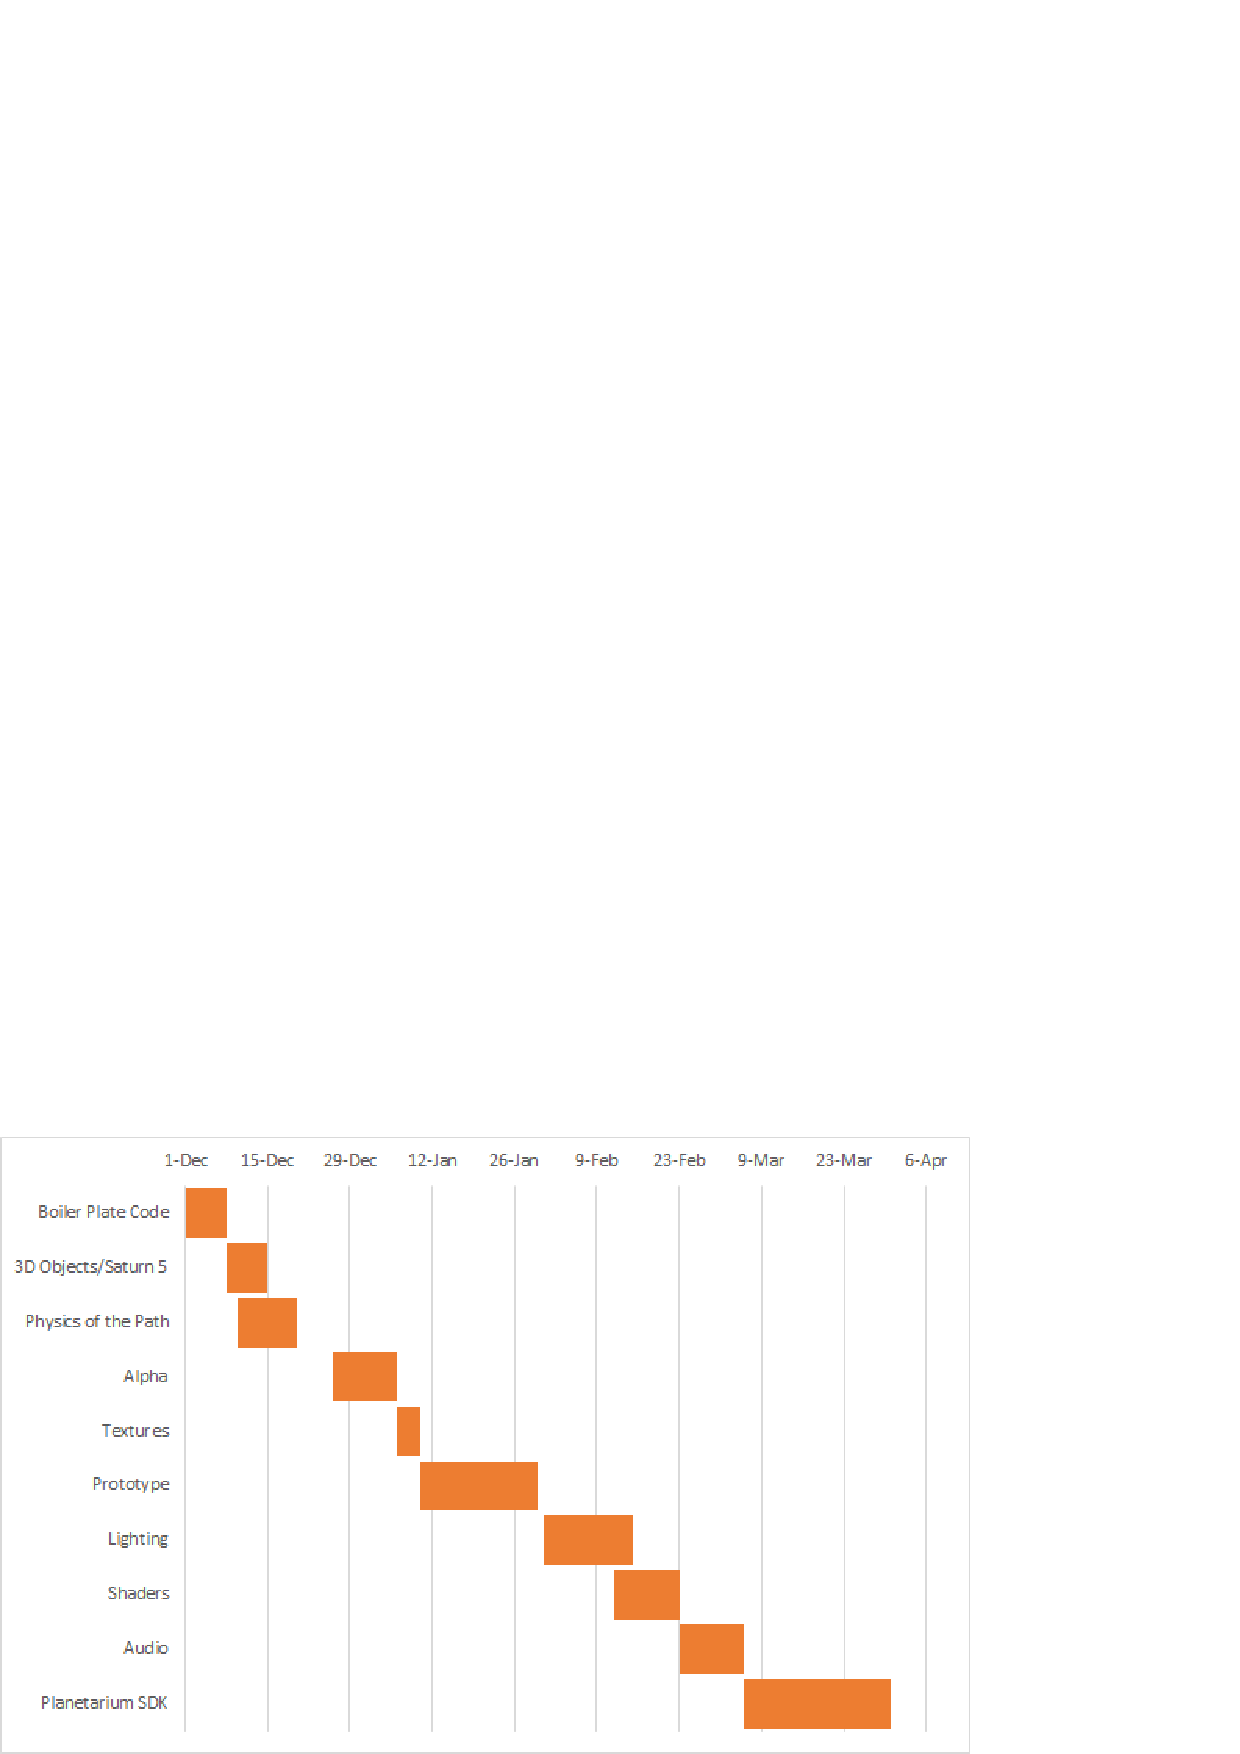
\includegraphics[width=\linewidth]{Gantt.PNG}
    \caption{Original gantt chart of proposed timeline}
    \label{fig:Gantt Chart}
\end{figure}


%%%%%%%%%%%%%%%%%%%%%%%%%%%%%%%%%%%%%%%%%%%%%%%%%%%%%%%%%%%%%%%%%%%%%%%%%
%%%%%%%%%%%%%%%%%%%%%%%%%%%%%%%%%%%%%%%%%%%%%%%%%%%%%%%%%%%%%%%%%%%%%%%%%
\section{Design Document}

\begin{titlepage}
    \begin{singlespace}

\includegraphics[height=2cm]{OSU_horizontal_2C_O_over_B.eps}   
        \par\vspace{.2in}
        \centering
        \scshape{
            \huge CS Capstone Design Document \par
            {\large\today}\par
            \vspace{.5in}
            \textbf{\Huge\CapstoneProjectName}\par
            \vfill
            {\large Prepared for}\par
            \Huge \CapstoneSponsorCompany\par
            \vspace{5pt}
            {\Large\NameSigPair{\CapstoneSponsorPersona}\par}
            {\large Prepared by }\par
            Group\CapstoneTeamNumber\par
            % 5. comment out the line below this one if you do not wish to name your team
            \CapstoneTeamName\par 
            \vspace{5pt}
            {\Large
                \NameSigPair{\GroupMemberOne}\par
                \NameSigPair{\GroupMemberTwo}\par
                \NameSigPair{\GroupMemberThree}\par
            }
            \vspace{20pt}
        }
        \begin{abstract}

        % 6. Fill in your abstract   
    
The Summer of 2019 will be the 50th anniversary of the Apollo 11 moon landing and our group, `The Apolloers', is working to create a 3D animation of the mission. This animation is being made for Jim Todd at OMSI so the animation can be displayed as part of their 50th anniversary exhibit. This document will show how we have organized the project and offer different design viewpoints so that stakeholders can see how the project has been structured. 

        \end{abstract}    
    \end{singlespace}
\end{titlepage}

\newpage
\pagenumbering{arabic}
%\tableofcontents
\subsection*{Revisions}
\begin{tabular} {|p{4cm}|p{5cm}|p{6cm}|}
\hline
Section & Original & New \\ \hline
3.5.2 - The Flight Path & \begin{itemize}
  \item We will use a data set to create the flight path
\end{itemize} & \begin{itemize}
  \item A data set would be ideal, but we will need to create our own
\end{itemize}\\ \hline
3.5.3 - Planetarium SDK & \begin{itemize}
  \item Unsure of how to show our animation in the planetarium
\end{itemize} & \begin{itemize}
  \item OMSI uses a unique scripting language for implementation in the planetarium
\end{itemize}\\ \hline
4.2 - Composition & \begin{itemize}
  \item Go through mission from launch to splashdown
\end{itemize} & \begin{itemize}
  \item Beginning and end with historic video, middle for interactive views
\end{itemize}\\ \hline
4.4 - Dependency & \begin{itemize}
  \item Mostly dependent on flight path and mission time
\end{itemize} & \begin{itemize}
  \item Dependent on the story-line that we created (Beginning, middle, end)
\end{itemize}\\ \hline
4.5 - Information & \begin{itemize}
  \item Focused on flight path information
\end{itemize} & \begin{itemize}
  \item How to make the scene realistic through size and positioning
\end{itemize}\\ \hline

\end{tabular}

% 7. uncomment this (if applicable). Consider adding a page break.
%\listoffigures
%\listoftables
\clearpage

% 8. now you write!

\subsection{Overview}
       \subsection{Scope}
        This document focuses on the 3D animation for the Apollo 11 Mission that will be created by our group, "The Apolloers" for display at OMSI. The design principals of the project will be outlined here, as well as design elements, such as functionality, usability, and requirements. These principals and elements will outline the deliverables of our project as well as the resources needed to complete it. The context, stakeholders, and intended audience our project will be used in will also be outlined, which will provide supplementary reasoning for our chosen delivarables. 
        
    \subsubsection{Purpose}
        The design and structure of this project will be outlined so that readers would be able to understand how the 3D animation is organized from a development viewpoint. In addition to the readers, this document will also serve as guidelines for our group to follow throughout the year. This document will be changed throughout the year as we refine our design. 

    \subsubsection{Intended Audience}
        This document is intended for the stakeholders of the Apollo 11 3D animation, as well as any interested group that would like to know more about how the animation is structured. Some main takeaways of this document are the design, structure, and connectivity of the components of our animation, so that readers would have a general idea of how to make a similarly structured project. 

\subsection{Definitions}

\begin{tabular} {|l|p{13.5cm}|}
\hline
Term & definition \\ \hline
API & An Application Programming Interface is a set of protocols and tools that are used to build a software application. Essentially the `building blocks' that a programmer uses to build an application.  \\ \hline
Apollo 11 Mission & A spaceflight operated by NASA to land the first humans on the Moon, launched July 16th, 1969.  \\ \hline
Graphics Pipeline & A conceptual model that describes the steps that a graphics system needs to perform in order to render a 3D scene. \\ \hline
High/Low Poly & The amount of polygons used to make a 3D model, impacting performance.\\ \hline
NASA & The National Aeronautics and Space Administration is a federal agency that focuses on research and development related to air and space.	\\ \hline
OMSI & The Oregon Museum of Science and Industry, located in Portland, Oregon	\\ \hline
OpenGL & An open-source graphics library API that is used to interact with graphics hardware to design 3D renderings.	\\ \hline
SDK & A Software Development Kit is a set of tools that program developers use to write programs for an application. \\ \hline
Polygon Count & Refers to the number of polygons in a scene. The more polygons in the scene, the more time it takes for the scene to be executed, often resulting in lag. \\ \hline
SkySkan & A company that provides planetarium software and equipment to OMSI. \\ \hline

\end{tabular}

\subsection{Design Description}

    \subsubsection{Design Stakeholders}
    The stakeholders for our project are OMSI, as well as the audiences who will be viewing our video. The educational and technical quality of our video will reflect on OMSI. The planetarium audiences will also be affected by the technical and educational quality of our video. If the video is more entertaining than educational, then the audience will not understand the impact and ambition of the Apollo 11 mission. If the video is more educational than entertaining, then the audience will be bored and less likely to pay attention to the content of the video.
    
\subsubsection{Design Views}
    The Apollo 11 animation project can be broken into different views that can all be used to describe the animation. This document will look at the design of the animation through the different viewpoints listed below, and will explain those viewpoints in detail in Section 4. 
    
    \subsubsection{Design Viewpoints}
    \begin{enumerate}
        \item \textbf{Context}: In what context will this animation be viewed.
        \item \textbf{Composition}: How the animation is separated into different entities.
        \item \textbf{Logical}: What logic is constant throughout the animation, regardless of design decisions.
        \item \textbf{Dependency}: How different entities of the animation depend on others.
        \item \textbf{Information}: What data will be needed and how it will be used in the animation. 
        \item \textbf{Interface}: How developers should correctly use the animation.
        \item \textbf{Resources}: What external entities are needed for the animation. 
    \end{enumerate}
    
    \subsubsection{Design Elements}
    There are many elements of a 3D animation that all need to work with the other elements to produce a quality project. The programming platform OpenGL will be used for managing the elements relating to 3D graphics. Since we are building for a Windows platform, we will also make use of Windows system calls as needed.
    
    The programming in OpenGL will dictate what 3D objects are in the project, where they are in the scene, and how they look. Many 3D objects in our project will come from an online repository, which we may need to add textures to, which would also be found online. Since the source for each object will likely be different, proper scaling will need to be applied to keep the size realistic. Once a 3D object is in the scene, different lighting features will be programmed in to account for the Sun and that light reflecting off of the other objects. Then to make objects move, key-frame animation will be used to interpolate the path between a start and goal point. 

    \subsubsection{Design Overlays}
	
	\subsubsection{Textures and 3D Models}
	Textures will be needed for some of our 3D objects, such as the Earth and Moon. Most of these textures will come from the NASA websites, which are readily available for public use. It is notable that these textures have been created with great detail, meaning that the textures may slow the program, or look out of place if near a lower quality texture. 
	
	The 3D model of objects such as the Lunar Module will likely be obtained from a model sharing site. We will attempt to find low-poly objects for our initial program so that the playback is not slowed down. High-poly objects may look better, but take many more resources to load. When our program is implemented at OMSI, Jim Todd should have industry quality models that can be used in the planetarium with less concern for polygon count. 
	
	\subsubsection{The Flight Path}
	Ideally we would want a dataset of the whole flight and back. Using that data set, paths can be interpolated from between the sets of points, resulting in a realistic flight path. While this would be straight-forward to implement, it is unlikely that we will have access to such a resource. Instead, we will need to calculate our own flight pat. This will still be done by using data points, but we must calculate each one, so there will be far less data points, meaning a less accurate flight path.
	
	\subsubsection{Planetarium SDK}
	One of our biggest stretch goals is to integrate our animation into the OMSI planetarium. We suspect that their planetarium use an SDK to interpolate subsections of the projection, but we currently do not have access to that SDK. Our contact here at OSU, Mike Bailey, has been in touch with SkySkan to determine how to best go about the process to implement an animation. It appears that there is a unique scripting language that is used for the planetarium. If the animation will go to the planetarium, we will use sample scripts to develop a prototype script resembling our animation for Jim Todd to test and finalize. 
    
    \subsubsection{Design Rationale}
	The basic rationale of our project is that setting the scene correctly is the most important factor in making this animation high quality. The Earth, Moon, and Sun need to be in the right position and the view port needs to be in the right position to reflect that. The lighting from the sun needs to be accurate as it reflects and refracts off the lunar capsule, Moon, and Earth. The small details matter the most, such as the Earth having its iridescent glow that is given off by its atmosphere, or both planetoids having a dark and a light side. With all of this combined, our goal is to make the audience feel as if they are watching the Apollo 11 mission live.
	
    \subsubsection{Design Languages}
	C++ is going to be our design language solely because of our choice to use OpenGL as our API. OpenGL makes use of graphics libraries that are written in C++, meaning that we must also utilize that same language. C++ gives the programmer great control over what they implement, but because of that control, this allows the programmer to make a lot of mistakes. C++ is fast and efficient like its predecessor language, C, and has more back-end libraries that can help the programmer achieve what he is trying to do. Even though these extra libraries can slow down an application, the effect is minimal for a project with a scope as large as ours. Lastly, our group will need to be cautious with memory usage because C++ does not automatically clean up memory such as some other languages, so we will need to be sure to free any memory that we allocate. 


\subsection{Design Viewpoints}

    \subsubsection{Context Viewpoint}
    
    This animation will be viewed primarily by OMSI visitors. This audience can range from young school children on field trips, to very technical industry leaders. We will want the user of this program to be able to change the viewpoint of the scene, regardless of if the user is a visitor or a staff member running the program.  
    
    \subsubsection{Composition Viewpoint}
    
    Our project will consist of a beginning, middle, and end. The beginning and end will consist of historic video related to the Apollo 11 mission to educate and provide context. The middle will allow the operator to take control of what viewpoint to see and be able to look around that view with the mouse. 3D objects, animation, audio, textures, lighting, shaders and more will all come together to create the scene. While there are not direct relationships between all these parts, they all add to the overall detail and quality of the animation. 
    
    \subsubsection{Logical Viewpoint}

    Our logic will be determined by how far into the animation the operator is. The beginning and end of the animation will be shown in a sequential fashion with little to no variation. When a certain action completes and/or a time is reached, new actions will take place. Conversely, during the middle of the animation, our program will allow changes in viewpoints. The simple logic will result from different keyboard buttons being pushed. These presses will not only change the view, but reset the previous and new scenes, this way the operator will always know what to expect when they press those keys. A stretch goal would be to allow some animations to be returned to the point in time when the last view was changed. This would be useful for a longer animation that the operator may want to pause and come back to later. 
    
    \subsubsection{Dependency Viewpoint}

    Different parts of the animation will not need to be loaded for certain viewpoints. For example, the lunar surface with an astronaut does not need to be loaded if the view is from the Earth. Each object will be given a 'flag' of sorts that we can set depending on what each view needs loaded. This will help with performance and prevent objects appearing out of place. Along these same lines, certain audio clips will be played when a view is chosen or when a certain time is reached. 
    
    Other than when to load objects, our program will not contain many actions that are dependent on others. With a graphics project such as this, all assets are loaded into memory at the beginning of running the animation so that each asset can quickly be retrieved for display to the screen. The program mainly determines when and how to display data from the computer's memory. 
    
    \subsubsection{Information Viewpoint }

    General knowledge of the Apollo 11 mission is needed to create an accurate representation in an animation. The sequence of events and a timeline are necessary, but also details such as the true size of all objects in the scene and the positioning of those objects. Because of our audience, extra care must be taken to make the animation as realistic as possible since there may be members of the audience that are quite knowledgeable about Apollo 11. When possible, all information will be acquired from an official NASA source and if that is not possible, other reliable sources will be used, such as news outlets and scientific journals. 

    \subsubsection{Interface Viewpoint}
    
   The 3D animation will be compiled into an executable file (.exe) so that the user can open the whole animation from one file. Then, the user will be able to start and stop the animation using a keyboard, and change their viewpoint by clicking and dragging their mouse, or choose set viewpoints using the keyboard. If the user does not want to change the viewpoint, the viewpoint will be set to default viewing positions that our group has chosen. The user will be able to view the video from outside of the spacecraft, inside the spacecraft, on the moon, and on Earth. 

    \subsubsection{Resources Viewpoint}
    To obtain the audio of the transmissions between the Apollo 11 crew and Tranquility Base, we will use NASA's archive of audio files from the Apollo 11 mission. Using Windows system calls, these files will be played approximately at the same stage of the mission as they were recorded in. Our group will not be implementing every audio file in the Apollo 11 audio archive, but instead we will aim to enhance the animation. The audio clips will need to be educational, but not include too much jargon for the audience. 

    Similarly to audio, our group will also need to obtain 3D models and textures from online repositories. Models will include the Command Module Columbia, and Lunar Module Eagle, an astronaut, and more. Multiple textures will be needed for the Earth and the Moon at different levels of detail, depending on how close the view port is during the animation. Finally, the background will need an accurate star-map to emphasize the vastness of space. Although, the star map needs to toggle because the stars cannot be seen from the surface of the Moon. 
    
\subsection{Conclusion}
A 3D animation consists of many different elements that all need to work together based on the implementation in a given API. We will be using OpenGL as our primary API that will manage the main graphical elements of our group's Apollo 11 3D animation. The animation will include historical context of the mission and what the mission was like on the Moon with full functioning elements such as 3D objects, texturing on those objects, lighting for the scene, etc. With a completed animation, direct users of the animation will be able to use a mouse and keyboard to navigate through the animation and view the scene through arbitrary viewpoints. Lastly, the main goal of this Apollo 11 animation is to engage audiences at OMSI and encourage curiosity in regards to the vastness of space. 

%%%%%%%%%%%%%%%%%%%%%%%%%%%%%%%%%%%%%%%%%%%%%%%%%%%%%%%%%%%%%%%%%%%%%%%%%
%%%%%%%%%%%%%%%%%%%%%%%%%%%%%%%%%%%%%%%%%%%%%%%%%%%%%%%%%%%%%%%%%%%%%%%%%
\section{Tech Review - Dean Akin}

\begin{titlepage}
    \pagenumbering{gobble}
    \begin{singlespace}
        \hfill 
        % 4. If you have a logo, use this includegraphics command to put it on the coversheet.
        \includegraphics[height=4cm]{OSU_horizontal_2C_O_over_B.eps}   
        \par\vspace{.2in}
        \centering
        \scshape{
            \huge CS Capstone Technology Review - Dean Akin \DocType \par
            {\large\today}\par
            \vspace{.5in}
            \textbf{\Huge\CapstoneProjectName}\par
            \vfill
            {\large Prepared for}\par
            \Huge \CapstoneSponsorCompany\par
            \vspace{5pt}
            {\Large\NameSigPair{\CapstoneSponsorPersona}\par}
            {\Large\NameSigPair{\CapstoneSponsorPersonb}\par}
            {\large Prepared by }\par
            Group\CapstoneTeamNumber\par
            % 5. comment out the line below this one if you do not wish to name your team
            \CapstoneTeamName\par 
            \vspace{5pt}
            {\Large
                \NameSigPair{\GroupMemberThree}\par
            }
            \vspace{20pt}
        }
        \begin{abstract}
        % 6. Fill in your abstract    
        	Our group, The Apolloers, is working with Mike Bailey to create a 3D animation about the Apollo 11 Moon Landing. This animation will be put on display in OMSI during the Summer of 2019 for the 50th anniversary of the Apollo 11 mission. All parts of the mission will be included, from Earth Launch to Earth landing, and all sections in between. This document breaks the project into requirements that we will use to guide our project through the development process. 
        \end{abstract}     
    \end{singlespace}
\end{titlepage}
\newpage
\pagenumbering{arabic}
%\tableofcontents
% 7. uncomment this (if applicable). Consider adding a page break.
%\listoffigures
%\listoftables
\clearpage


% 8. now you write!
\subsection{Introduction}
Every great animation has several objects that had to be sculpted and made for the scene , and we will have to do the same for our Saturn 5 model and several other objects to set our scene. The sculpting/modeling software we use is the real question, and each one has their pros and cons. the three options below is ones we may use.

\subsection{Blender} 
One of the more popular modeling softwares, it is mostly known for it being free, and the great community that backs this software. This is quite attractive to our group due to the fact we have very little budget, this automatically puts Blender as one of our choices. The other reason is because it has such a massive community, someone might of already made the Saturn 5, alot people in the Blender community have made just about anything you could think of, because of this, this could remove some of the time from making the model, to applying the Saturn 5 directly into the scene and going straight into the animation.
\subsubsection{Feature Rich!}
Blender is open-source, and because of that, feature development is is quick to be finished, and Blender has been out for awhile now. It has many features that one would heavily use when modeling anything, this includes rigging, fluid simulations, UV mapping, and more, and even has full fledged animation imbedded into it as well. It's interface is quite easy to use, and applying textures to a Saturn 5 shuttle would be much easier there than in OpenGL, the animation is a little hefty and we are not very familiar with the software itself, we can only apply the fundamental aspects to 3D modeling to Blender instead of using Blender at its full potential.
\subsubsection{Robust Hot-Key Workflow}
Blender sports a very robust hot-key system, which allows you to almost completely control blender through the keyboard. This means that if we learn the hot-keys for the things that we are doing, our working speed will become much faster. Blender also allows you to customize the control presets, if you wanted to set up Blender to be just like Maya or Max, you can, the Maya and Max control presets for example allow you to set up Blender just like Maya and Max with the same shortcuts and viewport navigation.
\subsubsection{Constant Updates, Massive Free Plug-In Library, and the Community}
One of the best things about Blender is that it is constantly updated, and because its constantly updated, its plug-in library is massive. You will find a plug in for just about anything you are doing, and not only that, the community also contributes various plug ins to the collection. What all of this means is that Blender is a software that is feature rich, and if we can use features that can make our job easier, we will use them, and Blender makes it very easy to make that happen. 
\subsubsection{Conclusion}
Even with all these features, Blender is very small and portable, and very extensible. Because it is this way, it can run on almost all operating systems, and on very low end hardware. To top it all off, it has everything we need to do a professional job, despite no company backing and lacking of the very latest technologies in 3D and animation. This makes it a very easy choice for us to pick. The only thing that is against us is the very clunky interface, and we still need to learn the software itself. Overall this may be the best pick for us due to the fact that its free, it has the features we need to finish our model quicker, it may even have a community that has created the model already, and has a community that is available to us to solve any problems we may have. 
\subsection{Maya}
Maya is one of the most popular 3D animation and modeling programs in the history of computer graphics. In fact, it’s so widely used that probably everyone with eyes has been exposed to something designed with Maya software. Maya is usually known for being the best at animation, in comparison to Autodesk's other design software, 3DS Max. It's easier to make realistic animation and effects with Maya. Maya also has incredible motion-capture handling, this making it the first choice for the film industry. Maya has a free-form approach to 3D modeling: instead of using only modifiers, you can apply modeling layers.
\subsubsection{Free-form UI}
Maya has a central tools pane at the top, but it divides its options more granularly (such as geometry, lighting, etc).  Maya is a little more free-form with its modeling: there is less dependence on modifiers, and modeling layers can be applied to the project and mixed a necessary. Holding space bar brings up a myriad of options and operations that can be selected, allowing for quick navigation through the UI. This could help us with being new with the software, and can help us with creating the model. 
\subsubsection{Nurbs Modeling}
Nurbs modeling, or Non-Uniform B-Splines provides a 3D modeling framework that is based on geometric primitives and drawn curves. Primitive are simple 3D objects that are created in the shape of common geometric forms such as cubes, spheres, cones, and so on. Primitives can be a great starting point for many complex 3D shapes. You can modify the attributes of NURBS primitives to modify their shape. You can also modify NURBS primitives by trimming away portions of their forms, beveling their edges, or by sculpting them into different shapes using sculpting tools that is native with Maya. This can be in our favor when making the model, the Saturn 5 is no simple 3D object. 
\subsubsection{Better Human Modeling}
Maya also has various small tools that make human modeling and animation that makes it more fluid. Most people swear by the poly tools that they're the best, this includes nHair, Soft Body Dynamics, Fur, Fluid Motion, Muscle Dynamics, and so on. Maya is known for better high-poly scultping tools, and better tools for animation and rigging. In terms of this project, non of this really applies to what we are trying to animate, because none of what we are doing requires us to mess with human movement, it more involves orbital mechanics and setting the scene. 
\subsubsection{Conclusion}
Maya seems to be the more powerful animation tool, and we could do the whole project in Maya. But the trick here is that alot of the tools are more tailored to character animation than what we would be using it for. Also, Maya is not free, and because of the budget, this kinda turns this away from being an option. Maya also has a much higher skill curve than Blender, which means we need to spend much more time learning the software than actually using it towards our project. Maya also doesn't have as big of a community of Open Source creators, despite it being one of the more popular 3D modeling softwares out there. Like Blender, it has a rich plug-in library which we could use to make our job go much faster. We are most likely not going to use Maya because it isn't the right fit in terms of our project, we need more precise tools than what Maya offer, something that is more user friendly up front.  
\subsection{3Ds Max}
3Ds Max software is a product by Autodesk , it is implemented across the Architectural , Engineering and Construction (AEC) industry to perform Architectural 3D modeling , it can perform 3D Mechanical modeling , 3D Architectural rendering , Exterior and 3D Interior walk-through and 3D Architectural fly-through. Autodesk 3Ds max is used by alot of video game developers and many TV commerical studios due to ability to use alot of movie effects. It has modeling capabilities and a flexible plugin architecture and it can be used on Microsoft Windows platform. Besides being used for engineering industry feats, this software has a wide range of usage for media and advertisment. 
\subsubsection{Rendering Capabilities}
3D max software has strong rendering capabilities, improved interoperability with industry-standard products as well as the additional time-saving animation and mapping workflow tools , it can add animated people with Populate and lots of small fixes. 3D max software has better viewport performance, it has perspective match tool, better particle system, vector map support, and it can work with other programs, such as Maya, Mudbox, and unity to name a few. It also has a better interface than Maya, it offers some tools and modifiers that are very easy to use, making our job much easier to do. 3D max is used for games while Maya is used for film work, 3D Max has better modeling tools , while Maya has better animation tools.
\subsubsection{Vector Map Support}
Vector map support is also a new feature , 3Ds Max enables the users to load the vector graphics as the texture maps , the users can render these texture maps at dynamic resolutions, the graphics will remain the same and clear if these graphics are zoomed-in effectively. This especially is good for us when it comes to making the model for the Saturn 5, than actually doing it manually, this allows use to kill two birds with one stone.
\subsubsection{Game Creation Ability}
ds Max helps users create massive game worlds, produce detailed characters, and customize building environments. They will be able to animate individual characters and make scenes that contain many people. The software allows them to simulate the physical properties of liquids like water, oil, and lava. In addition, 3ds Max has animation controllers that users can create, modify, and share. This can also be used for plotting the path of the Saturn 5, 3Ds max is used for more conceptual modeling, and if we can get a better grasp on what we are doing, doing the actual animation will be much easier.
\subsubsection{Conclusion}
Like Maya, 3Ds Max has a price tag, and this deters us from using 3Ds Max, and it isn't a small price tag. Although 3Ds Max is a better match for us than Maya for what we are going to use it for, it still doesn't seem to be the best match. It has alot of tools that we aren't going to use, so Blender would be are most likely choice. 
\subsection{Conclusion}
With everything considered, Blender seems to be the best choice for us. With a price tag of free, a vast library of tools, and a less steep learning curve, this would be the best for us to use.

%%%%%%%%%%%%%%%%%%%%%%%%%%%%%%%%%%%%%%%%%%%%%%%%%%%%%%%%%%%%%%%%%%%%%%%%%
%%%%%%%%%%%%%%%%%%%%%%%%%%%%%%%%%%%%%%%%%%%%%%%%%%%%%%%%%%%%%%%%%%%%%%%%%
\section{Tech Review - Jonathan Ropp}

\begin{titlepage}
    \pagenumbering{gobble}
    \begin{singlespace}
        \hfill 
        % 4. If you have a logo, use this includegraphics command to put it on the coversheet.
        \includegraphics[height=4cm]{OSU_horizontal_2C_O_over_B.eps}   
        \par\vspace{.2in}
        \centering
        \scshape{
            \huge CS Capstone Technology Review - Jonathan Ropp \par
            {\large\today}\par
            \vspace{.5in}
            \textbf{\Huge\CapstoneProjectName}\par
            \vfill
            {\large Prepared for}\par
            \Huge \CapstoneSponsorCompany\par
            \vspace{5pt}
            {\Large\NameSigPair{\CapstoneSponsorPersona}\par}
            {\Large\NameSigPair{\CapstoneSponsorPersonb}\par}
            {\large Prepared by }\par
            Group\CapstoneTeamNumber\par
            % 5. comment out the line below this one if you do not wish to name your team
            %\CapstoneTeamName\par 
            \vspace{5pt}
            {\Large
                \NameSigPair{\GroupMemberOne}\par
                %\NameSigPair{\GroupMemberTwo}\par
                %\NameSigPair{\GroupMemberThree}\par
            }
            \vspace{20pt}
        }
        \begin{abstract}
        % 6. Fill in your abstract    
        	This document aims to compare OpenGL, Unity, and DirectX to see what programming platform our group will want to utilize when creating our 3D animation of the Apollo 11 mission. After the comparison, we have determined that we will be using OpenGL because it offers more control over low level graphics and because our group has already had experience developing with OpenGL. We may also utilize Unity to create a final deliverable because of better options for after effects and bundling the project together. 
        \end{abstract}     
    \end{singlespace}
\end{titlepage}
\newpage
\pagenumbering{arabic}
%\tableofcontents
% 7. uncomment this (if applicable). Consider adding a page break.
%\listoffigures
%\listoftables
%\clearpage

% 8. now you write!
\subsection{Introduction}
Our goal is to create a 3D animation of the Apollo 11 Moon Landing, including all parts between the launch and the final splashdown. This animation will be displayed in the Oregon Museum of Science and Industry (OMSI) for guests to view in the planetarium. There are many different pieces to this process such as creating the 3D objects, using physics to simulate motion, lighting of the objects, how to handle audio, and much more. My role is to compare what programming platform we will be using for most of the project. In this document, the OpenGL, Unity, and DirectX development platforms will reviewed and compared to choose what will be best for our project. The review will be based on some brief history of each system, how each platform would be able to support our needs, how easy it would be for our group to learn, and how accessible the final project would be.

\subsection{OpenGL --- ``The Industry's Foundation for High Performance Graphics''}
OpenGL is a graphics library (hence the GL) introduced in 1992 and soon became the industry standard for 2D and 3D graphics applications [1]. OpenGL is currently operated by The Khronos Group, a non-profit consortium that works with similar open standard systems [2].  Open standards mean that the standard of the product is available to the public and is often favored in software development because of the extra control developers can have, especially when it comes to development on multiple different systems (Windows, Linux, mobile, etc.). This also means that there are many Application Program Interfaces (API's) that have spawned from OpenGL, such as WebGL, a variant that allows for graphics rendering within web browsers [3].
\newline
\newline
Since OpenGL is a collection of graphics libraries, using this in our project would essentially be a C++ program that utilizes these libraries, and other libraries as needed. Working with the libraries at this level gives access to make changes at a low level (close to the hardware). This is a great advantage for custom options, but it also means that there are few “shortcuts” that can be made, so programming can be quite tedious. However, for our group specifically, we are all currently taking CS 450: Intro to Computer Graphics, taught by Mike Bailey, our OSU lead for the project. In this class, we are learning how to utilize OpenGL which means that we all have similar experience with this platform and would not require learning many more concepts. 

\subsection{Unity –-- ``The World's Leading Real-Time Engine''}
Unity Technologies ApS (formally Over the Edge I/S) was founded in 2004 and is most well-known for their development of the Unity Real-Time Engine [4]. This engine is focused on creating 2D and 3D graphics that are then placed into an environment that developers can further manipulate, giving the term ``real-time'' engine. Unity provides a graphical user interface (GUI) for developing projects so that instead of just writing code, developers have graphical menus they can use to make changes. These interfaces are also useful for artists to customize visuals, and writers to change the general ``flow'' of the project. Unity is most known for being the engine that runs ``Half of the world's games'' and for good reason since Unity is available for every major system available today [5].
\newline
\newline
Unity is an ``engine'', meaning that a lot of overhead is handled for the developer behind the scenes. This can be great for developers that do not want or need to access to low level changes and it also helps to prevent overwhelming new users when they are learning how to utilize the system. This combines with the GUI to provide a streamlined interface that is still incredibly powerful. For groups, Unity also offer built in version control systems and cloud storage [5]. This allows projects to be stored and edited in the cloud, and all those changes are documented across the group. This service is free for groups of 4 or less, but bigger groups will have to pay monthly fees. While the Unity engine is free for people to use, because Unity is run by a for-profit company, other useful programs within the engine need to be purchased through a monthly subscription [6]. 

\subsection{DirectX –-- ``Are you excited? You will be''}
The first version of DirectX was released in 1995 and has had many different versions, up to DirectX 12 that was released in 2015 [7]. DirectX is a collection of API's that is included with Microsoft Windows to handle all multimedia tasks, especially 2D and 3D graphics. Notable API's include Direct3D, DirectSound, DirectInput, DirectDraw, and many more. DirectX has been the main graphical driver for Microsoft Window's operating systems and Microsoft Xbox systems with little to no compatibility with other systems. Even though DirectX is still staying strong with Microsoft, it appears that support for DirectX 12 has been dropping for other, multi-system options such as the Vulkan API, especially when it comes to the video game industry [8].
\newline
\newline
The DirectX software development kit (SDK) is made of runtime libraries that are a layer of abstraction up from direct graphical implementations [9]. While developers will still need to understand the basics of computer graphics, DirectX will handle some of the details automatically. This being said, due to competition from other low-level API's, DirectX 12 introduced low-level programming to the system so that developers could make low-level changes to reduce driver overhead [10]. Another area that DirectX has received pressure is the fact that it only runs on Microsoft Systems. Even though it does this very well, current trends in favor applications that can be run on many different systems. 

\subsection{Comparison}
We will start by comparing OpenGL and DirectX as these are the most similar. OpenGL provides more low-level options for optimizing graphics so that they can look the best while using as few resources as possible. While DirectX 12 has introduced similar low-level programming, there are still many factors that are handled by the DirectX API itself, which can help introductory developers, but may gloss over some details. Both systems would look similar in the eyes of a developer as they would be programming in a C-style environment to take advantage of graphics libraries/API's. However, one of the most notable differences is that OpenGL is open-source (and therefore works on many different systems) while DirectX is limited to Microsoft supported systems. In today's world, with so many different sysems such as macOS, Linux, Android, IOS, etc., multi-system support is a crucial feature to have when developing multimedia graphics. 
\newline
\newline
Comparing Unity and OpenGL is more difficult because OpenGL is a collection of graphical libraries, while Unity is a graphical engine, that manages many API's, that are based on libraries. This means that OpenGL will offer much more low-level customization while Unity offers a much more user-friendly environment to bypass the low-level options that may not be important to a larger program. Unity offers an easy to use GUI so that even introductory developers can get a foothold in their project without being overwhelmed with low-level code, while OpenGL requires the developer to write code for every aspect of their graphics project. With this being said, Unity still offers low level options to customize, but often the system will take care of that for the developer. Unity also makes importing other resources much easier because of the graphical interface. OpenGL requires separate libraries and functions to include resources such as sound, but again, offers complete control over these resources. Another factor with our project is the fact that all members of our group have had recent experience with OpenGL and can use Professor Mike Bailey as a resource for OpenGL support, while we have very little to no experience in Unity and would have to learn to use the entire engine. 

\subsection{Conclusion}
All the above options, OpenGL, Unity, and DirectX, would be suitable for our 3D animation of the Apollo 11 Moon landing. However, with our limited information about how OMSI will want to implement this animation, our group will not be using DirectX because it is not supported on a wide variety of systems. Between OpenGL and Unity, our group will primarily be using OpenGL based on our experience with the system. Also, implementing the physics for the different 3D objects will be best done on the low-level system. However, once the 3D animation is complete, our Group may still utilize Unity for after effects, adding audio to the presentation, and making a deliverable that is easy to use. It is too early to guarantee this, but the tools that Unity offers could make combining all our resources together much smoother than trying to program every aspect in OpenGL. In the end, our main goal is to produce a deliverable to be shown at OMSI and then shared with others, so as the project progresses, our group will use whichever systems we can to best achieve this goal. 

\subsection{References}
\begin{enumerate}
\item [1] Group, K. (2018). OpenGL - The Industry Standard for High Performance Graphics. [online] Opengl.org. Available at: \url{https://www.opengl.org/} [Accessed 31 Oct. 2018].
\item [2] The Khronos Group. (2018). The Khronos Group. [online] Available at:\url{https://www.khronos.org/} [Accessed 31 Oct. 2018].
\item [3] MDN Web Docs. (2018). WebGL: 2D and 3D graphics for the web. [online] Available at:\url{https://developer.mozilla.org/en-US/docs/Web/API/WebGL_API} [Accessed 31 Oct. 2018].
\item [4] Bloomberg.com. (2018). Company Overview of Unity Technologies, Inc.. [online] Available at:\url{https://www.bloomberg.com/research/stocks/private/snapshot.asp?privcapId=241908542} [Accessed 31 Oct. 2018].
\item [5] Unity. (2018). Unity. [online] Available at: \url{https://unity3d.com/} [Accessed 31 Oct. 2018].
\item [6]Unity Store. (2018). Store - Unity Store. [online] Available at: \url{https://store.unity.com/} [Accessed 31 Oct. 2018].

\item [7]	Codingunit.com. (2018). The History of DirectX | CodingUnit Programming Tutorials. [online] Available at: \url{https://www.codingunit.com/the-history-of-directx} [Accessed 1 Nov. 2018].
\item [8]	Smith, R. (2018). Comparing Vulkan \& DX12 API Overhead on 3DMark. [online] Anandtech.com. Available at: \url{https://www.anandtech.com/show/11223/quick-look-vulkan-3dmark-api-overhead} [Accessed 1 Nov. 2018].
\item [9]	M. Satran, “Getting Started with DirectX Graphics,” Microsoft Docs. [Online]. Available at:\url{https://docs.microsoft.com/en-us/windows/desktop/directx} [Accessed 01 Nov. 2018].
\item [10]	Channel 9. (2018). Direct3D 12 API Preview. [online] Available at:
\url{https://channel9.msdn.com/Events/Build/2014/3-564} [Accessed 1 Nov. 2018].

\end{enumerate}

%%%%%%%%%%%%%%%%%%%%%%%%%%%%%%%%%%%%%%%%%%%%%%%%%%%%%%%%%%%%%%%%%%%%%%%%%
%%%%%%%%%%%%%%%%%%%%%%%%%%%%%%%%%%%%%%%%%%%%%%%%%%%%%%%%%%%%%%%%%%%%%%%%%
\section{Tech Review - Shannon Sandy}

\begin{titlepage}
    \pagenumbering{gobble}
    \begin{singlespace}
        \hfill 
        % 4. If you have a logo, use this includegraphics command to put it on the coversheet.
        \includegraphics[height=4cm]{OSU_horizontal_2C_O_over_B.eps}   
        \par\vspace{.2in}
        \centering
        \scshape{
            \huge CS Capstone Technology Review - Shannon Sandy \par
            {\large\today}\par
            \vspace{.5in}
            \textbf{\Huge\CapstoneProjectName}\par
            \vfill
            {\large Prepared for}\par
            \Huge \CapstoneSponsorCompany\par
            \vspace{5pt}
            {\Large\NameSigPair{\CapstoneSponsorPersona}\par}
            {\Large\NameSigPair{\CapstoneSponsorPersonb}\par}
            {\large Prepared by }\par
            Group\CapstoneTeamNumber\par
            % 5. comment out the line below this one if you do not wish to name your team
            %\CapstoneTeamName\par 
            \vspace{5pt}
            {\Large
                \NameSigPair{\GroupMemberOne}\par
                %\NameSigPair{\GroupMemberTwo}\par
                %\NameSigPair{\GroupMemberThree}\par
            }
            \vspace{20pt}
        }
        \begin{abstract}
        % 6. Fill in your abstract    
        	For this technology review, I will analyze technologies for audio aspect of the Apollo 11 3D video. The technologies must fulfill our group's requirements for audio captioning, audio management APIs, and sound effects. For each technology, I will describe its functionality, affordability, and accessibility and review how well it meets our group's requirements. I will choose the most affordable technology that meets the requirements described in this paper.
        \end{abstract}     
    \end{singlespace}
\end{titlepage}
\newpage
\pagenumbering{arabic}

\subsection{Introduction}
For our project, my role is to include audio files from the original Apollo 11 mission into our video. The audio will also need to be captioned for accessibility. Audio files from the original mission need to be included because my group aims to create a realistic and entertaining re-enactment of the Apollo 11 mission for the Oregon Museum of Science and Industry (OMSI). For this review, I will be examining technologies for audio captioning, audio management APIs, and sound effects libraries for audio that is not available in the Apollo 11 audio archive.

\subsection{Audio Captioning}
When the audio of the conversations between the Apollo 11 crew and Tranquility Base are included in the video, they will also need to be captioned. The technology used to communicate between the Apollo 11 crew and Tranquility Base was very poor compared to modern standards, so captions will be needed to understand the grainy audio. Captions are also required so that Deaf and Hard of Hearing audience members can experience this video to the fullest extent.

The captioning technology we select will need to display a transcript of the current audio file without any errors. The technology will also need to display the captions at the same pace as the audio and be visible to the viewer regardless of the current viewpoint. Our group would also want to avoid having to buy an expensive video editor software in order to create the captions.

\subsubsection{Hard-Coded Captions in OpenGL}
For our video,  our group could hard-code the captions with OpenGL. In order to do this, captions would have to be implemented after the audio is completely added to the video. In fact, captions would have to be implemented late in the creation process. Hard-coding the captions would mean that they would be part of the scene itself rather than added on top of the finished video by an editor.

By hard-coding the captions, we would be able to control where the text appears and lock it at a certain position in the scene for each viewpoint. The color of the captions can also be changed, which would allow us to color-code the different speakers in the audio file. The fonts and font size are limited, however. The available fonts are Helvetica and Times New Roman, neither of which are dyslexic-friendly. The available font sizes are 10, 12, and 18 for Helvetica and 10 and 24 for Times New Roman [1]. Hard-coding the captions would also require our group to time the audio files and keep track of how long the captions need to stay on the scene before transitioning to the next set of captions. This method would be tedious and take time away from developing other aspects of the video.

\subsubsection{Unity Text UI}
The text interface for Unity allows for flexibility in captioning. The captions act as layer on top of the scene, allowing us to place the captioning independent of the scene. There is also a wide variety of fonts, font colors, and font sizes available. This would allow us to color-code the captions depending on whether Tranquility Base or the Apollo 11 crew are speaking. Custom fonts can even be imported to Unity and there is also an option to change the font's material. The alignment and overflow of the captions can easily be adjusted with Unity's interface as well. 

Using event triggers in Unity, our group would be able to trigger the captions to play when each audio file begins [2]. Instead of having to time the entire video and figure out when each line of every caption should be displayed, we would have to time every audio file and decide when to transition the captions.

\subsection{Audio Management APIs}
Under the assumption that our group will be using OpenGL to create the video, we will need to import audio management APIs because it does not have any audio support. The audio management API we select will need to allow us to change the volume of the audio files depending on the current viewpoint. We would also need the API to work on a variety of platforms, so the video can work properly in the OMSI planetarium. Our group would also like to avoid paying any licensing fees for the API.

\subsubsection{OpenAL}
One API we could use is Open Audio Library, or OpenAL. This free library's functionality closely resembles that of OpenGL, which would be beneficial for our group since OpenGL is the graphics program that we have the most experience with. In fact, the official website for OpenAL claims that anyone with experience with OpenGL will know how to utilize their library. The three basic objects in OpenAL are a Listener, a Source, and a Buffer. Buffers contain audio data and there can be multiple Buffers in a scene attached to one or more Sources. Sources represent the points in a 3D space that the audio is emitting from. Listeners represent the positions where the Sources are heard and there is only one Listener object present.


OpenAL allows for audio data to decrease and increase depending on the location of the Listener. This is especially beneficial for our team because we want to implement this functionality in our video. Also, almost 100 video games are credited with using OpenAL, including games that have been produced and distributed by major publishers such as \textit{Bioshock}. This helps lends credibility to OpenAL's performance. OpenAL implementation is also available on a variety of platforms such as Mac OS X, Linux, and Microsoft Windows. This means that our video could be played on a variety of operating systems without problem [3].


\subsubsection{IrrKlang}
IrrKlang is a sound engine and audio library that can be used in C++, meaning that it is also compatible with OpenGL. However, irrKlang is only free for non-commercial use. Since we plan for our video to play in the OMSI planetarium, we would most likely have to pay to use irrKlang. IrrKlang is platform independent and runs on operating systems including Windows 8 and 10, Linux, and Mac OS X. This would allow for our video to be viewed on a variety of platforms without problem. 

For each audio file, irrKlang allows the user to define a radius from which the audio will be heard and establishes each audio at a position in 3D space. IrrKlang also has no limit for the amount of audio files that can be included in a scene. Since irrKlang allows the user to increase and decrease the volume of the audio depending on where the listener is, this would allow our group to decrease the volume of the Apollo 11 crew transmissions whenever the viewpoint is outside of Apollo 11 [4]. 

\subsubsection{FMOD Studio Low Level API}
The FMOD Studio Low Level API allows for audio data to be placed in a 3D space. For each frame of the scene, the position and velocity for the listener object is set. Depending on the listener object's distance from the audio data and its velocity, the volume and pitch of the audio will increase or decrease [5]. For our video, we want for the volume of the Apollo 11 crew transmissions to increase when the viewpoint is inside the Apollo 11 and decrease when it is not. Currently, our group does not want to alter the pitch of the audio data, since that could cause the audio to be difficult to hear by the viewer.

The FMOD Studio Low Level API is available for a variety of platforms including Linux, Mac OS X, and Windows. The API also has a plug-in for Unity, so if our team decides to use Unity instead of OpenGL, we could use the same audio API regardless. Over 2,000 video games are credited with using FMOD API, including games that have been produced and published by major publishers such as \textit{Witcher 2}. However, it is unclear which video games are using the FMOD Studio Low Level API or the more complex FMOD Studio API. This may lend some credibility to the API's performance. It is unclear if our team would have to pay a licensing fee. The official site for FMOD states that if a video game developer has a budget of less than \$550,00, that developer is allowed to use their products for free for one game per year. However, if the products are not being used for a game, the developer must contact the company to receive a custom licensing fee [6]. Since our group is creating a video for OMSI, it is possible that we would have to pay a licensing fee.

\subsection{Sound Effects}
While our group has access to the archive of audio files from the Apollo 11 mission, these audio files only include the communication between the Apollo 11 crew and Tranquility Base. For our video, we intend to include other sounds such as the roar of the Saturn 5 launch and the splash of the splashdown to Earth. While it is possible to try to recreate these sounds, we are currently searching for an audio library that contains these sounds. These audio files will need to sound accurate and not like a cartoon sound effect. Much like the previous technologies, our group would like to avoid paying a licensing fee.

\subsubsection{FMOD.io}
FMOD.io contains a large library of audio files created specifically for sound effects in video games. In order to access this library, our group would need to download FMOD Studio. In addition to any licensing fee, we would need to pay 99 cents for each audio file that we download. FMOD.io allows the user to preview every audio file before they purchase it, so we would be able to determine which audio files would be realistic enough for our video.

FMOD.io organizes the audio files by categories based what genre the audio might be used for. This would help our group easily search for the audio files we need. Since this library was created for video game sound effects, we would be able to trigger the audio files to play at certain points in the video [6]. For example, we could script a trigger event so an audio file would play when the Saturn 5 begins to launch. Since FMOD Studio has a plug-in with Unity, we could also use FMOD.io if our group decides to use Unity to create our video.

\subsubsection{Noise for Fun}
Noise for Fun is a website created by a sound designer and composer that contains a variety of free sound effects. The website organizes audio files by categories that help identify the genre of the sound. Tags are also used to help further describe each audio file. Users can also listen to each audio file before they download it, so we would be able to confirm if the audio file sounds realistic enough to use in our video.

Noise for Fun is still in beta, so the utility of the site may not be as refined as other professional sites. One issue we may have with the site is finding realistic sound effects. The creator has stated that comical and fantasy sound effects are prioritized, so it may be hard to find audio files that depict a realistic "splash" sound during the splashdown in our video [7].

\subsection{Conclusion}
To add captions to our video, our group will hard-code the transcriptions in OpenGL. While the Unity UI Text has significantly more freedom and options when adding text to a scene, our group is planning to create the Apollo 11 mission video in OpenGL. I believe that the Unity UI Text is more user-friendly and would require less scripting, but we do not plan to use Unity to create our video.

For our audio management API, our group will use OpenAL. Unlike the other API's, OpenAL will be free for our group to use. OpenAL will also allow us to decrease and increase the volume of our audio files depending on the current viewpoint. The creators of OpenAL also claim that anyone who knows how to code with OpenGL will know how to code with OpenAL. This will be beneficial to our team since we have the most experience using OpenGL to create 3D graphics.

In order to obtain the audio files that are not included in the NASA audio archive of the Apollo 11 mission, our group will use the files available at Noise for Fun. While I believe that FMOD.io would offer more realistic and better quality audio, it would be significantly more expensive to use it. With Noise for Fun, we would be able to  download all the necessary audio files for free. 

\subsection{Citations}
[1] M. Kilgard, \textit{10.1 glutBitmapCharacter}, 23-Feb-1996. [Online]. 
\newline
Available: https://www.opengl.org/resources/libraries/glut/spec3/node76.html. [Accessed: 02-Nov-2018].

[2] “UI Text,” \textit{Unity}. [Online]. Available: https://unity3d.com/learn/tutorials/topics/user-interface-ui/ui-text. [Accessed: 02-Nov-2018].

[3] Openal.org. (2018). \textit{OpenAL: Cross Platform 3D Audio.} [online] Available at: https://www.openal.org/ [Accessed 2 Nov. 2018].
 
[4] “irrKlang,” \textit{irrKlang - an audio library for C , C\# and .NET and high level 3D and 2D sound engine.} [Online]. Available: https://www.ambiera.com/irrklang/index.html. [Accessed: 02-Nov-2018].

[5] \textit{FMOD Low Level API - An Overview.} [Online]. 
\newline
Available: https://www.fmod.com/docs/api/content/generated/common/lowlevel\_introduction.html. [Accessed: 02-Nov-2018].

[6] \textit{fmod.com}, 2018. [Online]. Available: https://www.fmod.com/. [Accessed: 02-Nov-2018].

[7] F. Vicarelli, “Free Sound Effects for Download at NoiseForFun.com,” \textit{NoiseForFun.com}, 2012. [Online]. Available: https://www.noiseforfun.com/. [Accessed: 02-Nov-2018]
\clearpage

%%%%%%%%%%%%%%%%%%%%%%%%%%%%%%%%%%%%%%%%%%%%%%%%%%%%%%%%%%%%%%%%%%%%%%%%%
%%%%%%%%%%%%%%%%%%%%%%%%%%%%%%%%%%%%%%%%%%%%%%%%%%%%%%%%%%%%%%%%%%%%%%%%%
\section{Blog Posts}
\subsection* {Dean Akin's Blog Posts}
\begin{longtable} {|p{1.5cm}|p{13.5cm}|} \hline
Fall: Week 4 &
As of right now we have finished our full problem statement, the main issue that we had to overcome is to make a good performance metrics section that portrayed it well, before we didn’t know how to write it. Due to time constraints and family issues on my part I was unable to meet with them Friday but nonetheless we finished it over google docs/github. We plan on meeting with Mike to go over requirements for our project next week. \\ \hline

Fall: Week 5 &
All we have to do is do our requirements document, everything is going pretty slow as of right now. Next week it will pick up. \\ \hline

Fall: Week 6 &
Tech reviews took awhile but all of them got done, still a slow week but documentation is always very small. Everything was smooth sailing for this week, we are planning on working together next week heavily on the design document, as planning correctly this term will decide how it will go next week.  \\ \hline

Fall: Week 7 &
The tech review didn’t take much, we are just waiting for the design document. \\ \hline

Fall: Week 8 &
We are currently hashing out the Design document this weekend, everything else seems to be okay. I am doing some pre-development for my final project for CS450 with Mike Bailey, as a proof of concept, and setting the scene. \\ \hline

Fall: Week 9 &
The only thing happening this week is working on the Requirements document over the weekend via pushing and pulling from github. Nothing else is happening due to a short week because of thanksgiving.  \\ \hline

Winter: Week 1 &
For progress we met up with Jim Todd at OMSI, he showed the WHOLE planetarium system and its API. We have a more solid understanding on what we want to do, and piping our animation into their system might of been easier than what we thought. We also met with some of the members of their research teams and asked for their opinion on what we should do and received feedback from them, and we headed home. No problems arised since then. We plan on starting development on storyboarding next week, other than that we are doing our required meetings.  \\ \hline

Winter: Week 2 &
We have managed to plan out certain things that we want to do at certain points of the animation. We have considered using key-frame animation as to have smooth interpolation of the ship and many other moving parts of the animation. Other than that we have been working on our elevator pitch and poster draft, not much has been going on. We plan to set the scene for the moon and to set up the work environment for our animation for further progress in the future early next week. \\ \hline

Winter: Week 3 &
We have drawn up a skeletal structure of our storyboard, and have decided which points in the animation can be interacted with and which are not. We have a clear goal on what we want to do to tell the best story that we can about the Apollo 11 mission, and next week we are planning to go into more detail on what we want to do within sub-scenes within the animation, and how we may do that. We are going to comprise what we wrote down into a document for Mike Bailey so that we can receive feedback on what we can further do to achieve what we want to do. \\ \hline

Winter: Week 4 &
Shannon is figuring stuff out on the audio/video stuff and the Lunar Module descent look at function. I am focusing on the key frame animation of Neil and lighting, and Jon is focusing on position of everything. As of right now, we are planning to delve more into the sound boarding than we did before. \\ \hline

Winter: Week 5 &
This week I worked on creating a key frame class while consulting Mike on what to do, during the meeting with Mike we also learned about the syntactic language that the proprietary software of the planetarium, and that Mike needs to write a MTL parser so we can read the material parameters for the objects which we loaded in. Other than that, we are tweaking position, rotations, etc, and plan on doing the same next week progressively. \\ \hline

Winter: Week 6 &
I continued on working ont he keyframe class, but ran into some issues. I cannot get it to reset so I am going to be working on that all week. \\ \hline

Winter: Week 7 &
We are finally able to get some headway on the project, I have finished per fragment writing and have been working heavily on the project while Shannon and Jon have been working on the progress report. Next week I will be working hard on the keyframe class implementation which is a big part of our project. Otherwise we keep going. \\ \hline

Winter: Week 8 &
Per fragment lighting is done, and I am almost done with the .mtl file parser to get the material parameters for the objects in the scene. Jon has gotten pretty much all of the big positioning done and Shannon has gotten something to work with the video. Next week I will be completing keyframing and animation so that things are moving. \\ \hline

Winter: Week 9 &
I am finally onto the lighting with the Earth, and how to combine all three textures into one. I have a general jist of what I want to do, but I have to write out what I specifically want to do.  \\ \hline

Winter: Week 10 &
I have finished some animation, as well as high res, blended texture of the Earth, to simulate the horizon in the original Earthrise picture during the Apollo 11 mission. For next week, I will be loading in the new lunar module/craft obj that we have received and will be adding some of our more common animations. Its basically cleaning up for the beta. No problems have arisen as of yet. \\ \hline

Spring: Week 1 &
I’m just finishing up Keyframing as it crashed magnificently, and then handing it off so Jon can do the flight path.  \\ \hline

Spring: Week 2 &
I finished keyframing and am working on an animation using it before the code freeze, otherwise all requirements are done and we just need to add more content. \\ \hline

Spring: Week 3 &
All I am doing this week is producing the wireframes of the animations I would like to do.  In the next following weeks I will do implement them and tweak them.  \\ \hline

Spring: Week 4 &
A test animation has been put up, but I am not sure why it very rigid in movement. Further investigation is needed, it is more than likely a simple error as it always is but we will see. Looking around in the animation moves smoothly. \\ \hline

Spring: Week 5 &
I added some in person perspective animations, and I am testing out why it seems so choppy. As of right now I am just adding more and more, soon I’ll get onto adding the textures onto the models. But that’ll be next week. \\ \hline

Spring: Week 6 &
I finally was able to move the eye position, and it was literally because of a type casting issue. Otherwise I’m adding all the animation as well as fine tuning performance on the animation.  \\ \hline

\end{longtable}


\subsection* {Jonathan Ropp's Blog Posts}
\begin{longtable} {|p{1.5cm}|p{13.5cm}|} \hline
Fall: Week 4 & 
We met with our TA, Richard Cunard, and got to bounce some ideas off of each other about how we are going to implement our 3D animation. Right after that meeting, we then met with our Client, Mike Bailey. We were able to get a few more details about the project and start thinking about what all we are going to need to start implementation. We started a shared document that is a list of things that we will need to know, and during our next meeting, we are going to discuss them and start breaking the list up into groups for us to work on. Lastly, we were able to finish our group problem statement and submit that assignment. Our biggest problem with that was that because our project is (objectively) straightforward, we put our document together and was still a bit short of the word count target. But, we were able to elaborate on a few portions and we look forward to getting the requirements document started. \\ \hline

Fall: Week 5 & 
This week we were unable to meet with our client, Mike Bailey, because they were out of town. We did still get to meet with our TA, Richard Cunard, and we were able to get some pointers for the requirements draft and the tech review draft. As a group, we met twice to work on the requirements draft, and finished it. Since the deadline was extended, we have not submitted so that we can have more time to read over it to check for errors and make additions.

We were seeming to have a bit of a hard time coming up with enough topics for the upcoming tech review draft. We were able to figure out the three sections that each of us will work on: How we are going to get/use 3D models, audio, and then what coding languages/interfaces we will use. Hopefully we will be able to look at these more and flesh them out before our next meeting so that we can discuss if we have any issues.

We plan to continue working on documents as assigned and meeting with our client/TA. Hopefully we will be able to review the requirements document with Mike next week to get his input. \\ \hline

Fall: Week 6 & 
This week we were able to meet with our client, Mike Bailey, and review our Requirements Draft. We received great feedback as well as having the opportunity to delve a bit deeper into some of the details of our project. We talked about everything from how audio of the mission was broadcast open mic, to the orbital mechanics that we will need to implement in our animation. Also, we discussed topics that each of our group members could write about for our tech review document; we decided to focus on the programming platform we will be using, and how to best integrate 3D objects and mission audio into the project.

Our group has still not had direct contact with our OMSI client, Jim Todd, and we brought that up with Mike. Mike offered to reach out to Jim and ask how involved with the process he would like to be, ranging from not at all, to sending technical documents and scheduling a trip to OMSI soon. Hopefully we will have a better idea about communication will look between our group and OMSI next week. \\ \hline

Fall: Week 7 & 
It has been a quiet week as our group has been working on finalizing our individual tech review documents. We were able to meet with our TA, Richard Cunard, and received more feedback on our requirements document, tips for the tech review, and a quick description of what our design document will be. After this, we were unable to meet with our client, Mike Bailey due to scheduling conflicts. We hope that early next week we can start getting an outline put together for our upcoming design document, getting advice from Richard and Mike. \\ \hline

Fall: Week 8 & 
As always, we met with our TA, Richard Cunard, and our client, Mike Bailey. With Richard, we discussed the layout for the design document that is coming up. We also learned about the 30 minute progress video that we will be needing to make by the end of the term. Then with Mike, we talked about what we learned in our tech reviews and that sparked conversations of development that will be great for our upcoming document. We have also heard back from our OMSI client, Jim Todd, through Mike, and Jim was happy with our design document. We hope to send Jim our design document and then after, all other documents for verification. Then lastly, our group is going to meet over the weekend to work on, and hopefully, finish the design document, as well as starting to set up our progress video. \\ \hline

Fall: Week 9 & 
With this being the week of Thanksgiving there is not too much to update. We were able to meet with our TA, Richard Cunard, and got a lot of clarification about our upcoming Design Doc. We also discussed the upcoming Client Verification and decided that we need to check in with Kevin and/or Kirsten to see if getting verification from Mike Bailey will be enough, or if we should try to get Jim Todd to sign off as well. Unfortunately, Mike had to cancel our weekly meeting, but we should be good to meet next week to cover the last two weeks of the term and what we should work on during Winter break. Our group has met to work on the Design Document and we have a decent outline, but we have a lot of details to add before we turn it in. Once that is done, we will start getting a plan for our progress video document and slides. \\ \hline

Winter: Week 1 &
During Winter break, our group, including Mike Bailey, drove to OMSI and met with our OMSI contacts, mainly Jim Todd. Jim was able to show us all the inner workings of the planetarium (Which was awesome!) and we got much more information about this project. This meeting was very good because I think that we all had something else in mind than what Jim had been thinking. This will mean that we need to go through all our documentation and change a decent amount, but all should be good.

We have scheduled weekly meetings with Mike for Fridays at 4 PM, and today we talked about our overall storyboard for the animation and some of the new goals that we should aim for. I think it really energized our whole team and we will start getting a basic scene put together for next week. Mike also let us know that he will be in touch with Sky-Skan (Planetarium software company) for more details of how we can possibly integrate an OpenGL project. Regardless of what will actually work with the planetarium, we will be making an OpenGL animation, at least to figure out positioning for our objects. \\ \hline

Winter: Week 2 & 
We met with Mike this week and we are still waiting on Sky Skan, but have only recently reached out. In the meantime, we are working on getting a general storyboard together for the animation. This will let us know what objects we need to load into the scene, where to place them and when. Also, a general story of the animation will be made so that we know what parts to focus on during viewing. 
\\ \hline

Winter: Week 3 &
This week we worked on finalizing our storyboard for our animation. We will run it by Mike for a final analysis during next week's meeting, but we have a solid idea of what story the animation will tell. During our meeting with Mike this week we talked about how to load in certain objects into OpenGL (Use blender to make things .obj). A small problem that came up is that Mike has still not heard back from SkySkan (planetarium software company) but that is not too critical. 

Our next goal is to get the lunar surface ready so that we can load in other objects and set the scene. We also discussed how to keep Jim Todd at OMSI updated and we will probably have one web meeting during the term about storyboarding and then make a trip to OMSI near the end of the term to test an alpha of the animation. 
 \\ \hline

Winter: Week 4 &This last week we worked to load in the lunar landing site and set up more of the scene. We also finalized our storyboard, though, after our meeting with Mike, we will likely re-format the storyboard to be more useful when setting up the OpenGL program. Also during our meeting with Mike, we found out that SkySkan has gotten back to Mike and they are excited to help out. It sounds like to display in the OMSI planetarium, we will need to use the software's unique scripting language, but after seeing some samples, it seems doable. We will still use OpenGL to plan out viewpoints and show a demo at Expo. 

Our main goal is to get an Alpha up and running for class. Some basics we want to include for this are all main objects loaded in the scene, some main viewpoints set up, and a general animation that navigates through the scene (Mainly the lunar surface and earth to moon). If possible, we would also like to load in a video and audio clip. 
\\ \hline

Winter: Week 5 & This week did not have any major updates as we are still working on getting an alpha ready. We did finally get to get a poster critique meeting and we got great feedback from Kirsten and group 72, we will focus more on what we created instead of the Apollo 11 mission. We also met with Mike again and he has gotten more info from SkySkan about scripting for the planetarium. For now, he is gathering all that and we are going to just focus on the OpenGL program for this term, switching to the scripting next term. 

This coming week is crunch time for the alpha. We need to finalize all positions, get lighting, get textures, get a demo animation path, and figure out how to load videos to OpenGL. We had assigned these parts to each of us and hope to get everything going this week. 
\\ \hline

Winter: Week 6 & 
Not much to tell this week other than continuing work on the Alpha. Work is going well with only problems coming up with incorporating video with OpenGL, but we are hoping to get help from Mike to make this a possibility. Overall, we should hit our goals for Alpha if work continues as planed. 
\\ \hline

Winter: Week 7 & 
Last week we were able to finish our Alpha with most of the features that we were aiming for (got stuck on playing videos and finding a flag object), but we are happy with it, as well as Mike. This week we all took some time for other classes but still are going to have our progress report finished by Monday. 

After our TA meeting, we did get more information about how we need to communicate our goals for the project. The OpenGL animation is a must-have for Expo, meaning that the script for the planetarium, while it is our main deliverable to OMSI, is going to almost be labeled as a stretch goal in terms of Expo and such. 

Meeting with Mike this week, we decided that we will try to make it to OMSI at the end of finals week and try to have some sort of simple script to try out to see if we are on the right page. We then reviewed what we need to get done for our beta and got a plan together for the rest of the term. 
\\ \hline

Winter: Week 8 & 
This week I worked on fine-tuning the positioning in the scene. Now the exact location of Tranquility base is marked and the Lunar Module is in the correct place on the lunar surface. Also, the Earth has been rotated to the correct angle as if you were on the Moon. Dean and Shannon have also worked on textures, key-frames, and audio.

My next goal is to figure out how to play video, which will probably give rise to some issues, but hopefully, I can get something working this week. Otherwise, we are still just working towards Beta. 
\\ \hline

Winter: Week 9 & 
This week our main struggle was with implementing video in OpenGL. We tried a few AVI libraries, ffmpeg, and OpenCV, and we ran into issues with all of them. After talking with Mike Bailey, we decided that play video at Expo was not a priority and that we should use that time to improve other parts of the project. 

In our meeting with Mike, we went over what we want to have done for our trip to OMSI at the end of the term (essentially for Beta). We need animated views and a cloud texture on the Earth. We also talked about other fine-tuning things (rounding the lunar surface, re-arranging things for viewpoints, LM texture). 

For the Lunar Module texture, we found out that all we have is color. This is a free object from NASA's Github, so we are considering purchasing one of better quality. Whatever we decide, the Lunar Module probably will not be textured for Beta, and we are fine with that. And lastly, we talked about documentation, updates to our poster, and questions to ask Jim at OMSI. 
\\ \hline

Winter: Week 10 & 
\\ \hline

Spring: Week 1 & While not much progress was made during spring break or this first week back, the Friday before break our team did drive to OMSI to meet with our client, Jim Todd again. Jim was happy with the progress we have been making and we put together a better plan for implementing our animation at OMSI's planetarium. But for now, we still need to focus on being ready for Expo.

Today we had our weekly meeting with Mike Bailey and went over what we need to do for this term. First, we want to essentially be ready for Expo by the code freeze. This would mean finalizing textures, more animations, and general fine-tuning. During this time, we would also make final changes to our documentation/poster. Then, we would shift our focus to creating the final project for use at OMSI. This will mostly take form of a unique script to be used by their Dark-Matter software. 
\\ \hline

Spring: Week 2 & This week we were unable to meet with Mike Bailey, but we plan to send our updated documentation to him for review. After we make any changes, we will send it to Jim Todd at OMSI. Also, since we could not meet with Mike this week so we do not have a system ready to read the texture associated with the new Lunar Module model that we got. So unfortunately it will not be ready for the code freeze, but all other aspect should be ready by Monday. 

Dean finished some animation code that we will get to work with this weekend and we are hoping to retrieve some more sources for audio and video clips. Lastly, the flight path needs to be finished and hopefully animated by Monday.
\\ \hline

Spring: Week 3 & 
This week was fairly quiet after getting the code freeze turned in. We made finishing touches to our documentation and sent it to Mike and Jim for verification. Unfortunately we have not gotten a response from Jim yet, but we will send a verified copy to Kirsten as soon as we do. We did still meet with Mike and we got feedback on our poster, then we went over a few more things that we need to do before Expo and then we divided up the work. We have some more animations to make and general fine-tuning of the project, but the next few weeks should be relatively slow before Expo. 
\\ \hline

Spring: Week 4 & 
This week we all continued work on additional animations and all individually ran into some delays. I have not found the best way to organize the animation for the flight path. Shannon is having issues with alpha masking the landing site. Dean's keyframes are not as smooth as they should be. Hopefully, these can be worked out in the coming week. 

We also made finishing touches to our poster and turned it in, but Mike still has not gotten the lunar module textures working, so we hope to have that finished after this weekend so we can add a textured screenshot to the poster before printing. 
\\ \hline

Spring: Week 5 & 
This week each of us made progress towards our individual animations. We also finished and submitted the final version of our poster for printing. We are feeling good with the expo and are hoping to have the project essentially done next week, that way we have a week to prepare for expo directly. 
\\ \hline

Spring: Week 6 & This week we all continued to prepare for the engineering expo next week. We worked with engineering IT to get a desktop computer to use with a 1080 ti graphics card. Our animation has been tested on this and is currently in Mike Bailey's office. This weekend, we plan to meet and produce the final animation for expo, along with any final preparations. 
\\ \hline

\end{longtable}


\subsection* {Shannon Sandy's Blog Posts}
\begin{longtable} {|p{1.5cm}|p{13.5cm}|} \hline
Fall: Week 4 & 
Progress: Our group has set up weekly meetings with Mike Bailey on Tuesdays, directly after our meetings with our TA. We met with our TA this week and discussed how our group can best move forward with our project. Our group also met with Mike Bailey to discuss our first steps for this project. Currently, we're collaborating on a list of what we will need in order to complete the video. This list includes: 3D objects with textures, audio files from the Apollo 11 mission, and details about the mission. We also have created a very rough timeline for our project.

Problems: There were not really any problems that we encountered this week. Our group was unable to meet in person to work on the group problem statement. However, we have been communicating over text regarding which sections we are each working on, so it was not much of a problem for us to complete the paper.

Plans: We plan to meet with Mike Bailey again on Tuesday with the completed list of what we need to complete the video. Our group is also planning on taking a trip this month to the Oregon Museum of Science and Industry to meet with our client, Jim Todd, and better understand what he would like from this video. No later than the beginning of winter term, our group plans to begin developing the video. By the end of January, we plan to have a prototype we can show our client so we can receive feedback\\ \hline

Fall: Week 5 & 
Progress: Our group was able to meet a couple times in person to work on the requirements document. On Wednesday, we finished a very rough draft of it and were also able to figure out what technologies we were going to do for the technology review. We also met with our TA on Tuesday to discuss what the requirements document should look like and also received guidance for the technology review. Our group also completed a list of what is required to be in the video and sent it to Mike Bailey.

Problems: Mike Bailey was out of town this week, so we were unable to meet with him to further discuss the requirements for the video.

Plans: We plan to proofread our requirements document and send it to our clients before we meet with Mike Bailey on Tuesday. When we meet with Mike Bailey, we also plan to discuss the technologies we should expect to use when creating the Apollo 11 video. \\ \hline

Fall: Week 6 & 

Progress: Our team was able to meet with our TA and Mike Bailey on Tuesday to go over the draft of our requirements doc. After the meetings, we made slight changes to our document that our TA and Mike Bailey suggested we make. This included adding the OSU logo, changing the name of our client for accuracy, and recreating our Gantt chart with Microsoft Project. In class on Tuesday, our group worked collaboratively to create our Team Expectations document. Mike Bailey also said that he would send a copy of our requirements doc to Jim Todd, our client at OMSI, and explain what the document represented. In our meeting with Mike Bailey, each of us went over what technologies we were planning to write about in our technology review.

Problems: There weren't really any problems this week. We were all able to make it to our meetings and worked collaboratively on the requirements doc and team expectations doc.

Plans: On Tuesday, we plan to meet with Mike Bailey and see if Jim Todd was able to get back to him about the requirements doc. We will also inform Mike Bailey of the technologies we decided to use based on our tech reviews. When we meet with our TA on Tuesday, we will go over what future work we should be preparing for. \\ \hline

Fall: Week 7 & 
Progress: We were able to meet with our TA on Tuesday and received feedback on what we should change for our final requirements document. We also discussed what the design document should be. We sent our revised requirements document draft to Mike Bailey so he can send it to our client, Jim Todd.

Problems: Mike Bailey was unable to meet with us this Tuesday because he had another meeting to attend at that time. Because of this, we were unable to go over what technologies we recommended using as a result of our technology review.

Plans: We plan to meet with Mike Bailey on Tuesday to go over what technologies we recommend using for our project. We will also meet with our TA to update him on our group's progress. We also plan to begin outlining our design document next week. \\ \hline

Fall: Week 8 & 
Progress: We were able to meet with our TA on Tuesday to discuss the requirements for our design document and progress report. We also discussed how we could more effectively complete these requirements. We were also able to meet with Mike Bailey and discuss what technologies we felt would be the best to use for our project. 

Problems: One of our teammates, Dean, was unable to attend both our meetings with Mike Bailey and our TA. We will have to update him on what we learned about our design document and progress report. We also don't know what 3D modeling technologies he recommended using for our project. We've also had trouble meeting as a group this week because none of our schedules aligned.

Plans: Either this weekend or on Monday, our team will meet to make a rough draft of our design document. While we all meet, we can fill Dean in on the information he missed from Tuesday's meetings. We will also ask him about what technologies he recommends for the 3D modeling in our video. We will also work together to find an accurate flight path of Apollo 11. Before the end of the term, Dean and I will complete 3D scenes that can be implemented in the prototype of our video. My scene will be of Apollo 11's splashdown and Dean's will include a model of the earth and its atmosphere as well the orbital mechanics will we need for out video. \\ \hline

Fall: Week 9 & 
Progress: Our team was able to meet last week to outline and draft our design document and go over what aspects of the paper each person will work on. We were also able to meet with our TA on Tuesday to clarify some confusions we had with the design document.

Problems: We were unable to meet with Mike Bailey on Tuesday because he had another meeting to attend. It was also hard for our group to meet this week because of the holiday break.

Plans: Our group plans to meet Sunday or Monday so we can finish our design document. We will also begin to outline our progress report as well. On Tuesday, we plan to meet with Mike Bailey to discuss how we plan to move forward with our project and to go over some aspects of our design document. We will also meet with our TA on Tuesday to ask any questions we may have about our progress report. \\ \hline

Winter: Week 1 &
Progress: Before the term started, our group and Mike Bailey visited OMSI to meet with our client, Jim Todd. We were able to discuss what scenes he wanted in the video and how the planetarium screens will distort the video. We have also set up weekly meetings with Mike Bailey for Fridays. After todays meeting with Mike Bailey, we discussed the story-boarding of the video and contacting NASA to use the 3D models from their Github. We have sent our TA our availability, but have not heard back from him yet.

Problems: We do not know if the planetarium video software can use an OpenGL program. Mike Bailey will be in contact with Skydance, the software company, to receive an answer.

Plans: We plan to set up weekly meetings with our TA. We also plan to begin working on the moon landing scene of our video this week.\\ \hline

Winter: Week 2 & 
Progress: Our group set up meetings with our TA for Wednesdays. During our meeting this week, we updated him about our meeting with our client and our updated expectations for our project. We also discussed how to prepare for our elevator pitch and poster board display. Our group met Friday to work on our project together. We began setting up the scene for the portion of our video that takes place on the moon. We have also signed up for the Engineering Expo and began work on our poster display draft.

Problems: We were unable to meet with Mike Bailey this week because he was out of town. Our group plans to use 3D models from NASA's Github for our video, but we will need permission from NASA to do so. Since Mike Bailey has a contact from NASA, he was going to help us gain permission to use the models. 

Plans: Our group plans to work together on Monday to finish up the moon scene. We will also work on using videos from the Apollo 11 mission as textures for our video. This will allow us to smoothly transition from actual footage from mission to our 3D video. 
\\ \hline

Winter: Week 3 &

Progress: Our group has met with our TA on Tuesday to discuss our progress with our video as well as what resources we will need for the Expo. Our group has also met with Mike Bailey on Friday to discuss how to use NASA's 3D models from their Github. We are now able to export these models has .obj files, making it so we can import them into our scene. This Friday, our group has also finished story-boarding our video and decided which scenes the viewer can interact with. Our group has also submitted our draft of our Expo poster.

Problems: Our group still has not heard back from Sky-Skan, the company responsible for the OMSI's planetarium software. So we still do not know if our OpenGL code will be compatible with the planetarium software. If the code is not compatible, we will need to write a script that takes the OpenGL code as input and alters it so it can be run by the planetarium.

Plans: We plan to meet with Mike Bailey next Friday to go over the storyboard of our video. Our group also plans to add NASA's 3D models to our scene and also implement more viewpoints. We also plan to review footage and audio of the Apollo 11 mission so we can see which files are suitable to use in our video.  
 \\ \hline

Winter: Week 4 &
Progress: Our team met with our TA to discuss what to expect for our alpha. Our scene has implemented the lunar module and landing site models into our scene and have also added textures for the sun and moon. We have also implemented some of the various viewpoints for video, including the viewpoint from the lunar module. Our team has also met with Mike Bailey, who had a chance to look through our storyboard. Mike Bailey also let us know that Skyskan (the company who created the planetarium's software) has replied to him. Unfortunately, the software will not take an OpenGL file. 

Problems: Our team will have to write a script so our video can be played in the planetarium. Luckily, the scripting language does not look too complex and Jim Todd has experience writing scripts for the planetarium, so we will reach out to him for support.

Plans: We plan to reformat our storyboard as an Excel sheet so we can write down how long each aspect of the video will be and keep track of the run time. We also plan to implement .mtl files to texture the landing site and lunar module objects. Our team plans to meet up next week to work on an alpha for our video.
\\ \hline

Winter: Week 5 & 
Progress: We met with our TA on Tuesday to discuss what was expected for our alpha and progress report. Afterwards, our team decided who will do what tasks so our alpha can be completed by Monday of week 7. I will be responsible for implementing the .mtl for our objects. I will also implement a sound file for our video. Our team met with Mike Bailey on Friday to update him on our progress as well as discuss what our alpha will look like. Our team met with team 72 to critique each others' posters on Friday morning.

Problems: Our team has not run into any problems with our project. If it snows this weekend that might prevent our group from working together on the project. However, we would still be able to work on the project individually.

Plans: Our team will keep working on the timing of our storyboard and the tasks that have been assigned to each of us. I will work on implementing OpenAL this week, the audio management library for OpenGL. We will also update our requirements document to better reflect our new requirements.
\\ \hline

Winter: Week 6 & 
Progress: Our team has completed our alpha for our project. I have also updated our requirements document to better represent our new requirements for our project. On Wednesday, our team met with our TA to confirm assignment due dates and update him on our project's progress. Our project now has a working audio byte, multiple viewpoints, and all the objects that will be in our video. On Friday, we met with Mike Bailey to update him on our progress. 

Problems: We did not encounter any problems this week. Our team was able to complete each task assigned to them for the completion of our alpha.

Plans: Our group plans to finalize the textures of the objects we retrieved from NASA's Github. We also plan to implement key-frame animation and more audio bytes in our video. We will begin to add historical videos in our project by adding them as 2D textures.
\\ \hline

Winter: Week 7 & 
Progress: On Wednesday, our group met with our TA to discuss future due dates and the expectations for our beta and progress reports. Our group has made a list of all the tasks that need to be done for our beta and have started working on them. On Friday, our group met with Mike Bailey to show him our finished alpha and also explain our progress to him. We told him that we will share our progress report with both him and Jim Todd. We also discussed visiting OMSI to show Jim Todd our beta. We are tentatively planning on going to OMSI on the Friday of finals week, if our schedules permit it. Our team also worked together on the progress report draft and finished most of it.

Problems: We have not run into many problems this week. Our group is still figuring out how to implement historical videos into our animation.

Plans: Our group plans to meet with our client either during or after finals week to show him our beta. We also plan to work on the animation, adding more audio, implementing the historical videos, finish texturing objects, and improving lighting.
\\ \hline

Winter: Week 8 & 
Progress: Our team met with our TA on Wednesday to update him on our progress and any problems that may arise by the end of the term. Our group also met with Mike Bailey on Friday to update him on our progress and to discuss techniques that may help us with what we are working on. Our group has made progress on the keyframe animations, the textures of our .obj files, making our scene more realistic and correctly scaling the scene.

Problems: Our team has not really run into any problems this week. We have yet to hear from Jim Todd if he will be available to meet at OMSI on the Friday of finals week.

Plans: The lunar surface should be correctly scaled and oriented along with the lunar module, astronaut, and American flag by the end of the weekend. We expect that the texturing of the .mtl files and keyframe animations will be completed soon after. We plan to spend the rest of the term working on adding historical videos and making it so users can break from the default video to view the scene from another viewpoint.
\\ \hline

Winter: Week 9 & 
Progress: We met with our TA on Wednesday to update him on our progress and also the problems we have been having with uploading videos as textures. The lunar surface object has been correctly scaled. Our group also met with Mike Bailey on Friday to update him on our progress and what we plan to do in the future. The flag has been textured and added to the scene, so all of our objects are now in the scene.

Problems: We are still having problems implementing videos as textures. We are currently looking for new solutions on how to execute this function.

Plans: With the lunar surface correctly scaled, we can focus on implementing it on the moon texture. When the user zooms in close enough, the lunar surface will be loaded on top of the moon and will be alpha-masked to blend in with the moon texture. We also plan to make the Earth look like it has clouds by implementing a fragment shader to add white noise to the Earth texture. The texture for the lunar module is close to being complete as well as the basic keyframe animation code. Once the keyframe animation code is complete, we will add multiple viewpoints to create our default animation. 
\\ \hline

Winter: Week 10 & 
Progress: Our team met with our TA on Wednesday to update him on our progress. We also met with Mike Bailey to demo our progress. So far, we have implemented keyframe animation, a mini map of the flight path to the moon, a more realistic looking Earth, animation of the lunar module landing, and have implemented more viewpoint and audio files that play during the scene.

Problems: We plan to meet with our client on Friday. Unfortunately, that means receiving feedback on the progress of our project after the beta has been finished.

Plans: We plan to implement a couple more viewpoints, more keyframe animations, and higher quality objects and textures.
\\ \hline

Spring: Week 1 &
Progress: Our group has set up weekly meetings with Mike Bailey for Fridays. We met with him today to update him on our progress and plans with the project as well as the timeline for Spring Term. We have reached out to our TA to set up weekly meeting with him. Our group is also working to set up a time where we can all meet and work on the project together.

Problems: We have not run into any problems at this time.

Plans: We plan to continue working on our project this weekend and next week so it will be Expo-ready by the code freeze. We also plan to send our updated documentation and poster to our client for verification. 
\\ \hline

Spring: Week 2 & 
Progress: Our team has made progress with the keyframe animations for our project. We have also updated our requirements documents to send to our client on Monday. We met with our TA today to discuss what is required of us for this next week.

Problems: Mike Bailey was unable to meet with us this week. Unfortunately, we were expecting to receive his higher-quality texture for the lunar module, so the lunar module's texture has not been applied yet.

Plans: Our group plans to animate the flight path, add more keyframe animations, and add more audio clips from the Apollo 11 mission. After these are implemented, we will have fulfilled our requirements for our project.
\\ \hline

Spring: Week 3 & 
Progress: Our team has completed everything we needed for the code freeze. We met with Mike Bailey on Friday to discuss what we have left to finish. We have finished our final version of our documentation and are still waiting for our client to verify them. We have made some edits to our expo poster.

Problems: We have not run into many problems this week. Our client has yet to verify our documents that we sent him last Saturday.

Plans: We plan to have the updated lunar module texture by the end of this weekend. I plan to work more on the alpha-masking for the landing site model and edit some audio files so they are not as long. Once the alpha-mask is finished, I will add an animation where the camera zooms in on the landing site. Our group plans to animate the flight path and add a default animation that explores the lunar surface.
\\ \hline

Spring: Week 4 & 
Progress: Our team has finished our poster for expo. We met with Mike Bailey on Friday to show him the progress on the flight path animation. The flight path now includes the return path Apollo 11 made back to Earth. We figured out that the landing site texture keys off X,Y coordinates instead of the S,T coordinates we were originally using. 

Problems: So far the only problem we have encountered is that we have not yet received the lunar module texture. We plan to receive it in the coming week.

Plans: I plan to edit the lunar module landing animations so they are more accurate to how the landing looked. I also plan to keep working on the alpha-mask of the landing site object. I will be cutting the audio clips down in length and also making it so they do not play during when the user switches scenes. Johnathan plans to edit the flight path so it does not rotate with the moon. Dean plans to edit the keyframe animation so the motion is smoother and less jumpy.  
\\ \hline

Spring: Week 5 & 
Progress: We met with our TA on Friday to discuss what to expect at Expo and what our booth needs to be ready. Our group also met with Mike Bailey to update him on our progress. The alpha mask for the landing site has been implemented and I have made it so the audio clips stop playing when the user changes scenes. Our poster and model release forms have been turned in.

Problems: We have not run into any problems this week!

Plans: Each team member plans to work on a key-frame animation scene. We plan to have them done a week before Expo so we are not rushing to finish them. After that, we will implement the higher quality texture for the lunar module.
\\ \hline

Spring: Week 6 & 
Progress: I have made the lunar module more accurate to how it actually happened. Dean and Jonathan had a meeting with Mike to update him on our progress and fill him in on the details about Expo. I was unable to make this meeting because I had a lab to attend for another class.

Problems: We have not run into any problems this week.

Plans: We plan to meet tomorrow morning to work on finishing the final details of the project. Dean will work on the default animation, Jonathan will work on animating the flight path, and I will trim down the excess audio and work on the landing site masking.
\\ \hline

\end{longtable}

%%%%%%%%%%%%%%%%%%%%%%%%%%%%%%%%%%%%%%%%%%%%%%%%%%%%%%%%%%%%%%%%%%%%%%%%%
%%%%%%%%%%%%%%%%%%%%%%%%%%%%%%%%%%%%%%%%%%%%%%%%%%%%%%%%%%%%%%%%%%%%%%%%%
\section{Poster}
\includepdf{Group49_Poster.pdf}

%%%%%%%%%%%%%%%%%%%%%%%%%%%%%%%%%%%%%%%%%%%%%%%%%%%%%%%%%%%%%%%%%%%%%%%%%
%%%%%%%%%%%%%%%%%%%%%%%%%%%%%%%%%%%%%%%%%%%%%%%%%%%%%%%%%%%%%%%%%%%%%%%%%
\section{Project documentation}

This animation was written using OpenGL and can most easily be built using Microsoft Visual Studios. A user would be able to open our solution (.sln) file in Visual Studios and compile the program. The program should automatically find the best Windows SDK to use, but if not, we compiled using version 10.0.17134.0 in Visual Studios 2017. Also, the OpenGL solutions must be built on a Win32 platform. As long as these settings are chosen correctly, a user should be able to debug and build the project. 

Once built, the program will run automatically, but will also output an executable file at "ProjectCode/Debug/Apollo11.exe" that can be ran without building again. Please note that depending on the machine this is being ran on, it can take a few minutes to load all the assets before the animation will start. Once the animation has loaded, the user will see usable keybindings on the screen, but here is a complete list: 
\begin{itemize}
\item Left-click and drag - Move scene
\item 0-9 - Change views 
\item E, W, Z - Additional views
\item F - Toggle flight path
\item L - Toggle lighting
\item M - Toggle text
\item Q - Quit animation
\item R - Toggle repeat animation
\item S - Toggle star map
\item +/- or scroll wheel - Zoom in/out
\end{itemize}

%'Project flow' here:


%%%%%%%%%%%%%%%%%%%%%%%%%%%%%%%%%%%%%%%%%%%%%%%%%%%%%%%%%%%%%%%%%%%%%%%%%
%%%%%%%%%%%%%%%%%%%%%%%%%%%%%%%%%%%%%%%%%%%%%%%%%%%%%%%%%%%%%%%%%%%%%%%%%
\section{Resources}

Our most valuable resource was Mike Bailey, our mentor and computer graphics professor here at Oregon State University. with his many years of experience with computer graphics, and specifically OpenGL, nearly all questions were answered by Mike. Additionally, our client, Jim Todd, gave us all the technical knowledge for the planetarium system at OMSI and how to implement a solution there. 

%Websites here
 
 
%%%%%%%%%%%%%%%%%%%%%%%%%%%%%%%%%%%%%%%%%%%%%%%%%%%%%%%%%%%%%%%%%%%%%%%%%
%%%%%%%%%%%%%%%%%%%%%%%%%%%%%%%%%%%%%%%%%%%%%%%%%%%%%%%%%%%%%%%%%%%%%%%%%
\section{Conclusion}

%Each of us answers:
%What technical information did you learn?
%What non-technical information did you learn?
%What have you learned about project work?
%What have you learned about project management?
%What have you learned about working in teams?
%If you could do it all over, what would you do differently?

\subsection{Dean Akin's Reflection}
I have learned alot from developing this project throughout the year. What I am most greatful for is that I truly got to learn in depth how graphics in general work, and how to go about making and developing stuff pertaining to it. I learned how to interrupt the pipeline and get into the nitty gritty just to get exactly what I wanted to happen, such as shaders and even developing my own technique to get what I want (Blending the 3 textures of the Earth together based off of a position) through my own understanding of how it all works. I also got to learn in depth the fundementals of fluid animation via keyframing by developing my own class that we could use for our own animation in the project. 
On the flipside, I learned a solid way to keep my development cycle organized and neat which I have struggled with before, this may be due to the group work environment or some other factor. This allowed me to finish something every week, and never stop at any point. It also made me excited to work on the project, as it feels good to know you've accomplished something and your one step closer to the finished result, which made me want to tinker with it more on my off time.
Project work is an interesting beast to experience. You're not only in charge of how your contribution works, but how it affects the others in your groups contributions. You need to be weary about what you're doing instead of getting it to work and shipping it. This also promotes a better product as it forces you to be more aware of what you're doing due to outside responses.
Dividing up the work and playing with eachother strengths really made this project move smoothly, and allowed us to learn from eachother more than if we were to struggle on something we truly are not suited for. Seeing how something works and looking how someone did it truly allows you to understand it than if you were to struggle to get it to work which could promote bad development practices.
In retrospect, I would more than likely divide my work up more evenly than I did. My organizational skills truly did excel at the latter half of the project development, as I started to get into a ritual of sorts. Other than that, I wouldn't change much.


\subsection{Jonathan Ropp's Reflection}
Working on a large-scale technical project taught me many things about my field, teamwork, and myself. Most of the projects I have done in the past have been short sprints, with this being the first lasting any more than a few months. That resulted in a new dynamic for me and one of the most important things I learned is how much more important good design is with a larger project. Along with that, making changes in the middle of a larger project have more implications, so it is important to make sure all members are on the same page with those changes. 

With our project in-particular, we all gained so many more skills relating to computer graphics. While we had all taken an introductory class with Mike Bailey, getting to apply what we learned to a large project took our understanding of computer graphics to the next level. Specific skills such as lighting, shaders, key-framing, and general object placement all came into play and gave us great practice. 

Looking back at this project, while I am happy with what we did, I do think we should have focused more on implementing our project at OMSI directly. We decided to take the skills we already learned and turn that into an animation for general computer, which worked well, but still left a lot of work left to get something for use at OMSI. Some of that comes down to some early communication problems we had, resulting in some differing expectations between stakeholders in the project, but overall, I still feel like we met our goals. 


\subsection{Shannon Sandy's Reflection}
While working on this project, I have gained significant technical and non-technical information. My knowledge of the graphics pipeline was strengthened and I have learned how to import .obj and .mtl files into an OpenGL program. I also became more skilled with writing GLSL shaders. I also learned how to play audio files in an OpenGL program as well as prematurely end thos audio files when a scene is changed. During the development of this project, I gained a deeper understanding of the importance of documenting requirements in detail. I also have learned more about what effective communication looks like within a team and with a client. Organization and time mangament where also skills that I strengthened while working on this project.

During the development of this project, I realized how setting weekly goals helped with meeting our larger project goals. Weekly meetings with my team also made it easier for us all to understand who is working on what aspects of the project and their progress. I feel I have also gotten better at adapting to and overcoming sudden changes that happen well into the development of the project. If I were to do this all over again, something I would do differently is get into contact with SkySkan earlier. This would allow us to have more time to learn the DarkMatter scripting language and also have a better idea of how the project will be implemented in the planetarium. I would also try and communicate with our client earlier so our team could have a clearer, more detailed understanding of our requirements before we start our requirements documents and project outline.


%\section{Appendix}
%Some code snippets?


\end{document}
